\documentclass{article}

\usepackage{cancel}
\usepackage{amsmath}
\usepackage[includehead,nomarginpar]{geometry}
\usepackage{graphicx}
\usepackage{amsfonts} 
\usepackage{verbatim}
\usepackage{mathrsfs}  
\usepackage{lmodern}
\usepackage{braket}
\usepackage{bookmark}
\usepackage{fancyhdr}
\usepackage{romanbarpagenumber}
\usepackage{minted}
%\usepackage{subfig}
\usepackage[italian]{babel}
%\usepackage{float}
%\usepackage{wrapfig}
%\usepackage[export]{adjustbox}
\allowdisplaybreaks

\setlength{\headheight}{12.0pt}
\addtolength{\topmargin}{-12.0pt}
\graphicspath{ {./Immagini/} }

\hypersetup{
    colorlinks=true,
    linkcolor=black,
}

\newsavebox{\tempbox} %{\raisebox{\dimexpr.5\ht\tempbox-.5\height\relax}}


\makeatother

\numberwithin{equation}{subsection}
\newcommand{\tageq}{\tag{\stepcounter{equation}\theequation}}
\newcommand{\vv}[1]{\verb{\text{#1}}}
\AtBeginDocument{%
  \renewcommand{\figurename}{Fig.}
}
\fancypagestyle{link}{\fancyhf{}\renewcommand{\headrulewidth}{0pt}\fancyfoot[C]{Sorgente del file LaTeX disponibile al seguente link: \url{https://github.com/00Darxk/Intelligenza-Artificiale-e-Machine-Learning}}}

\begin{document}

\title{%
    \textbf{Intelligenza Artificiale e Machine Learning}  \\ 
    \large Appunti delle Lezioni di Intelligenza Artificiale e Machine Learning \\
    \textit{Anno Accademico: 2024/25}}
\author{\textit{Giacomo Sturm}}
\date{\textit{Dipartimento di Ingegneria Civile, Informatica e delle Tecnologie Aeronautiche \\
Università degli Studi ``Roma Tre"}}

\maketitle
\thispagestyle{link}

\clearpage


\pagestyle{fancy}
\fancyhead{}\fancyfoot{}
\fancyhead[C]{\textit{Intelligenza Artificiale e Machine Learning - Università degli Studi ``Roma Tre"}}
\fancyfoot[C]{\thepage}
\pagenumbering{Roman}

\tableofcontents

\clearpage
\pagenumbering{arabic}

\section{Introduzione: Intelligenza Artificiale e Machine Learning}

L'intelligenza artificiale è l'area di studio che analizza come permettere ai computer di 
compiere operazioni che eseguite da un essere umano richiederebbero intelligenza. 
Rappresenta uno dei campi di ricerca più interessati recentemente ed ha avuto un'enorme 
crescita dal punto di vista economico e tecnologico. 

Un modo per poter riepilogare la storia dell'intelligenza artificiale consiste nell'elencare 
i vincitori del Turing Award, in questo campo. Questo premio rappresenta l'analogo del 
premio Nobel per l'informatica. 

\subsection{Storia dell'IA}

La prima fase di questa storia si può attribuire a personaggi come Alan Turing, che introdusse 
il concetto di ``test di Turing'' per determinare se una macchina si può considerare 
intelligente nel 1950. Una macchina secondo questo criterio si può considerare intelligente se 
un essere umano interagendo con essa, senza saperlo a priori, non sia in grado di sapere 
se si tratta di una macchina o di un altro essere umano. 

Un altro di questi personaggi fondamentali è John McCarthy, ha coniato il termine ``intelligenza artificiale'', 
nel 1955 ed ha proposto la creazione di un gruppo di lavoro l'anno successivo al collage di Dartmouth. 
Al convegno di Dartmouth del '56  parteciparono 
tutti i personaggi che vengono chiamati i padri fondatori dell'IA. 
L'obiettivo del convegno era lo studio della costruzione di macchine in grado di 
formare astrazioni e concetti, per risolvere problemi, al tempo riservati agli umani. 
In questo convegno si teorizzò che queste macchine potranno svolgere funzioni umane, 
ritenute intelligenti. 

In questo convegno Cliff Shaw, Allen Newell e Herbert Simon dimostrarono il primo 
programma di intelligenza artificiale, chiamato ``Logic Theorist'', in grado di dimostrare 
i teoremi dei Principia Mathematica. 
Proposero l'idea di ``General Problem Solver'' per risolvere una grande varietà di problemi 
simulando i processi mentali umani. 
Questo sistema riusciva a dimostrare teoremi, calcolare funzioni matematica e risolvere 
problemi logici. Da sistemi come questi si crearono grandi aspettative per l'intelligenza 
artificiale, in questa seconda fase tra il 1952 ed il 1969. 
In questo periodo Nathaniel Rochester all'IBM sviluppò tra i primi programmi di IA. 
Nel 1959 Herbert Gelernter scrisse il ``Geometry Theorem Prover'', capace di dimostrare 
teoremi matematici complessi. 
John McCarty nel 1958 all'MIT definì il linguaggio di lato livello Lisp, destinato 
a diventare il linguaggio di programmazione per eccellenza dell'IA per i seguenti trent'anni. 
Nel 1963 fondò il laboratorio dell'IA a Stanford, per costruire una versione 
definita dell'``Advice Taker''. 


Nonostante queste grandi aspettative, i sistemi di IA realizzati per problemi semplici 
non dimostravano un comportamento altrettanto soddisfacente per problemi di natura 
più complessa. 
Uno dei problemi per questo mancato successo dell'IA in questo periodo tra il '66 ed il '73 fu 
l'incapacità di comprendere l'intrattabilità di molti problemi, su cui l'IA stava cercando 
di operare. 
Nel 1973 venne stilato il rapporto Lighthill, dove venne criticata l'intelligenza artificiale 
per la mancata soluzione al problema dell'``esplosione combinatoria'', ovvero sull'utilizzo 
dell'IA per problemi di natura reale. 

Un altra critica giunse dal libro ``Perceptrons'' scritto nel 1969 da Marin Minsky e Seymour Papert 
che, come altri, discusse il limite fondamentale della struttura di base per generare un 
comportamento intelligente. In questo periodo il clima generale attorno all'IA era pessimista 
e libri come questo aiutarono a maturare questo clima di diffidenza nei confronti delle 
potenzialità dell'IA. 

Negli anni successivi per risolvere il problema dell'esplosione combinatoria si 
realizzarono sistemi basati sulla conoscenza, riservati ad esperti umani del settore. 
Questi programmi erano estremamente utili su settori molto ristretti, costituiti da un motore 
di inferenza. 
Il collo di bottiglia per questi sistemi era la conoscenza, per cui esistevano intere posizioni 
dedicate a trovare un modo per rappresentare ed astrarre il dominio di interesse su cui 
opera l'IA. Queste persone venivano chiamate scienziati della conoscenza, ed erano tipicamente 
professionisti ed esperti di quel settore specifico. 

Nel 1981 il governo giapponese avviò un progetto chiamato ``Quinta Generazione'' per realizzare 
computer intelligenti utilizzando il linguaggio Prolog. Analogamente sia gli Stati Uniti che 
l'Inghilterra finanziarono progetti simili. 

Tuttavia questi progetti non riuscirono a mantenere le loro promesse sulle capacità 
dell'IA o di impatto commerciale. I sistemi erano comunque limitati da una conoscenza limitata 
ed una difficile capacità di apprendere dall'esperienza e verificare la correttezza. Erano 
sistemi poco flessibili e robusti rispetto agli obiettivi promessi da questi progetti. 

Nonostante questo tra l'inizio e la fine degli anni '80 l'industria dell'IA conobbe un boom 
economico con centinaia di aziende costruttrici di sistemi esperti, di visione artificiale, 
di robot, di software ed hardware specializzati per questi scopi. 

Molte di queste aziende fallirono per l'impossibilità di mantenere le loro promesse e seguì 
un periodo chiamato ``inverno dell'IA'. 


A metà degli anni '80 almeno quattro gruppi diversi reinventarono l'algoritmo di apprendimento 
basato sulla retropropagazione, sviluppato negli anni '60. Questi modelli furono considerati 
in diretta opposizione ai modelli simbolici di Newell e Simon e dell'approccio logicista 
di McCarthy. 
Geoff Hinton è una delle figure in primo piano nel risorgere delle reti neurali durante 
gli anni '80 e 2010, descrisse i simboli come l'``etere luminifero dell'IA''. 

Dai limiti dei sistemi esperti si introdusse un nuovo approccio basato sulla probabilità invece 
che sulla logica booleana, sul ``Machine Learning'' più che sulla programmazione manuale, 
su risultati sperimentali più che su affermazioni filosofiche. Questo permette a questi 
sistemi con logiche non cablate di poter apprendere dall'esperienza e migliorarsi nel tempo. 

Nei primi anni del 2000 con lo sviluppo e l'espansione del ``World Wide Web'' ed il progresso 
sulla potenza di calcolo ha permesso di realizzare data set molto grandi, fenomeno 
indicato con il termine ``big data''. Questo ha portato allo sviluppo di algoritmi di machine 
learning progettati per trarre vantaggio da questi grandi insiemi di dati. 
La loro disponibilità ed il cambiamento di approccio verso il ML ha permesso all'IA di 
recuperare appetibilità commerciale. 


Nel 2006 Geoffrey Hinton, introduce un algoritmo di apprendimento veloce per reti 
neurali, dando il via alla rivoluzione del ``Deep Learning''. Utilizzando molteplici livelli di 
elementi computazionali il ML diventa Deep Learning. Questo sistema ha ottenuto successi 
in molti domini applicativi, aumentando l'interesse 
verso l'IA. 

Attualmente l'IA è in grado di lavorare in molti settori:
\begin{itemize}
    \item Può guidare veicoli robotizzati come automobili o droni autonomi. Nel 2004 DARPA introduce una sfida per la guida autonoma di veicoli;
    \item Permette di eseguire locomozione su arti con robot umanoidi;
    \item Pianificazione e scheduling autonomo, per la navigazione autonoma ed il sistema GPS globale;
    \item Traduzione automatica;
    \item Riconoscimento vocale;
    \item Raccomandazioni su social network per gli utenti. Nel 2006 Netflix ha lanciato una borsa per aumentare la precisione del loro sistema di raccomandazione tramite ML, vinta nel 2009;
    \item Può battere i migliori giocatori umani in molti giochi. Nel 1997 Deep Blue batte il campione del mondo di scacchi Garry Kasparov, e nel 2011 IBM Watson batte i campioni del gioco ``Jeopardy!'', ora questo sistema è utilizzato in molti sistemi. Tra il 2015 ed il 2017 AlphaGo di DeepMind batte i campioni del mondo nel gioco di Go, lo stesso team ha sviluppato AlphaZero in grado di giocare sia scacchi, shogi e Go;
    \item Può interpretare e riconoscere immagini. Nel 2021 ImageNet comincia il suo concorso annuale per rilevare e classificare correttamente oggetti in un set di immagini ampio e ben accurato, con un incremento nella precisione dovuto ai progressi nelle ``deep convolutional neural networks''. Nel 2014 Facebook pubblica un lavoro sul DeepFace in grado di identificare volti con un'accuratezza del 97\%;
    \item Permette di diagnosticare malattie, raggiungendo o superando la diagnosi di medici esperti;
    \item Recentemente ha accelerato la ricerca per il vaccino anti-Covid, nell'individuazione delle proteine utilizzate;
    \item Permette di rilevare informazioni dettagliate su eventi climatici estremi. 
\end{itemize}

Nel 2014 il consumo di energia per raffreddare i Data Center è stato ridotto del 40\% con un modello 
di ML, analogamente nel 2017 il software per analizzare le immagini di galassie sotto lenti 
gravitazionali è stato velocizzato di un fattore di $10^7$.  

Nel 2022 venne rilasciato ChatGPT, ``Generative Pre-trained Transformer'', il chatbot di OpenAI 
progettato per rendere efficace la comunicazione con un utente umano. 

\subsection{Il Machine Learning}

L'intelligenza artificiale è una disciplina molto vasta, non copre solo tematiche sulla ricerca di una 
soluzione ottima. Esistono sistemi esperti per effettuare decisioni, offrire raccomandazioni, aiutare nella 
programmazione. 

Dopo il 2006 le aziende hanno capito l'impatto che le raccomandazioni hanno nel mantenere l'attenzione del 
cliente e migliorare il loro servizio, quando Netflix ha annunciato un concorso di un milione di dollari 
per migliorare il suo programma di raccomandazioni del 10\%. Da allora tutte le principali aziende di 
investimenti, di viaggi, di intrattenimento, etc. Tutte le aziende che hanno di interesse l'interazione 
degli utenti. 

Ora è veramente di interesse, infatti la massima conferenza sulla ricerca SIGIR
``Special Interest Group on Information Retrieval'', prima trattava principalmente problemi di ricerca, 
mentre recentemente la sua attenzione si è rivolta su sistemi di raccomandazione. 

Un sistema di Machine Learning ML, all'interno di un dominio, dove ci sono dati validi con una loro 
consistenza, rappresenta un processo di apprendimento supervisionato o meno su questi dati per 
poter gestire e generalizzare i nuovi dati nello stesso dominio applicativo. 

Uno dei grandi passi avanti nel campo delle immagini si deve al grande dataset ImageNet, grazie ad una 
ricercatrice e professoressa di Stanford, che ha investito il suo tempo nel progetto. Questo insieme contiene 
milioni di immagini descritte e la loro classe di appartenenza dell'oggetto raffigurato, sono infatti 
principalmente immagini in primo piano. Tramite insiemi di dati come questi, il sistema apprende in un 
approccio supervisionato, poiché ad ogni immagine viene indicata la classe di appartenenza, ed in alcuni casi 
si indica dov'è presente l'oggetto nell'immagine. Date queste due indicazioni si possono creare sistemi di 
identificazione o individuazione di un'immagine. 
Questo approccio può realizzare sistemi di riconoscimento facciale, individuando le facce da un'immagine ed in 
seguito riconoscere le facce dall'immagine. 

La maggior parte dei dataset saranno supervisionati, ma esistono moltissimi dataset i cui data-point non sono 
indicati o descritti. Questo tipo di apprendimento prevede l'assenza delle classi dell'appartenenza, questo 
viene utilizzato per creare sistemi che possono essere in grado di identificare il rischio di una certa 
malattia, tramite delle caratteristiche comportamentali o genetiche. Oppure si assegnano a degli algoritmi 
di clustering un insieme di utente, che sulla base delle caratteristiche di quest'ultimi individua 
delle classi di utenti. Nel diagramma di dispersione dove sono presenti questi data-point si possono quindi 
individuare cluster diverse. Si utilizza questo approccio nelle comunità social per identificare 
comunità distinte. 

Se si trattano fenomeni fisici che non sono caratterizzabili a priori si effettuano degli studi per vedere se 
sono presenti correlazioni tra i data-point e quindi dei cluster, ed eventualmente individuare informazioni 
da questi dati. 

L'apprendimento per rinforzo è molto comune, ed è un sistema dove un agente interagisce con un ambiente, senza 
un dataset, per permettere all'agente di operare sull'ambiente, questo fornisce delle ricompense all'agente in caso 
effettui un certo tipo di azioni. Queste ricompense possono essere positive o negative, e sulla base di queste, 
si realizza il meccanismo di apprendimento. 
Alcune aree di dominio che si predispongono a questo tipo di apprendimento, dove sulla base delle ricompense 
si possono suscitare reazioni e quindi comportamenti desiderati dall'agente, sono i videogiochi. 

Grazie al DL si ha una sistema di ``Deep Reinforcement Learning'', dove il sistema è in grado di imparare 
direttamente da un'immagine, un video, uno spettrogramma, etc. 

Nel 2013 la DeepMind, di proprietà di Google ha dimostrato la possibilità di un agente di apprendere 
tramite DRL, su numerose partite di Breakout un comportamento ``super-umano'', e diversi altri giochi arcade 
della Atari. 
Un altro grande dominio dove questo tipo di approccio è utile è la robotica, dimostrato dalla Boston Dynamics 
e dal loro robot umanoide Atlas, in grado di camminare, saltare, portare pesi, su diversi tipi di terreni 
autonomamente. Il loro successivo robot Spot, ha risolto alcuni dei problemi, non dovendo imparare 
una locomozione su due piedi molto più complessa, basandosi invece sullo scheletro di un animale quadrupede 
come un cane. 


Il reinforcement learning venne introdotto per la prima volta una ventina di anni fa da Richard Button e Andrew Barto, 
degli psicologi cognitivi, senza tutta la serie di risorse di calcolo e di data per favorire questo approccio. 
Quindi non si è affermato per molto tempo. 

Nel 1997 venne proposta l'idea della RoboCup, un campionato di calcio composto da squadre di robot autonomi, 
da parte di diverse università entro il 2050, in grado di confrontarsi con la squadra di calcio campione 
al mondo. 

Il ML quindi ha l'obiettivo di generalizzare ed effettuare decisioni, il quanto più accurate, su un relativo dominio 
i cui dati non ha ancora visto. 


L'apprendimento è una componente chiave del ragionamento, ma non è sufficiente a generare IA in grado di 
generare nuova conoscenza. Tecniche di generazione del testo, delle immagini e musica, etc., sono note 
già da anni, ma solo recentemente con ChatGPT utilizzando una serie di tecniche che consentono un 
addestramento molto accurato ed efficiente su di un patrimonio di dati che è sterminato. 
Tutte le aziende informatiche, capiscono che questo è una minaccia, poiché permetterebbe di catturare 
oltre alla frequenza dei termini anche il loro contesto. Dal contesto è quindi in grado di determinare 
la probabilità che una certa parola appaia. 
Infatti ChatGPT è uno strumento statistico, poiché non ha alcun tipo di ragionamento, per questo si 
parla anche di allucinazioni, poiché non può creare nuova conoscenza, ma offre esempi dove lo strumento 
non rinuncia di predire, ma produce un risultato scorretto. 


Il processo di ML permetterebbe di realizzare software 2.0, tramite una rete neurale in grado di identificare 
le istruzioni da dover eseguire per effettuare una data azione, senza l'appoggio di un programmatore esterno. 
Questo solleva una serie di problematiche relativo ai pericolo del ML. 


Jeremy Howard ha esposto su una ``TED talk'' un problema analogo alla rivoluzione industriale in 
termini di occupazione, dove l'80\% delle persone lavora sui servizi, un dominio di interesse dove 
l'intelligenza artificiale è in grado di lavorare molto bene. Per cui quando questi sistemi entreranno 
a regime e le aziende si renderanno conto di questi strumenti così potenti a disposizione, allora 
sostituiranno questa occupazione umana, creando problemi occupazionali. 
Già nel 2015 nel concorso ImageNet, sullo stesso dataset, il tasso di errore di agenti intelligenti è sceso 
al disotto del tasso di errore umano nel riconoscimento delle immagini. Anche se l'essere umano è in grado 
di identificare in più classi distinte rispetto all'agente artificiale ed è in grado di contestualizzare 
queste immagine. 
Ma in alcune professioni quello che le macchine possono offrire, in termini economici, è più conveniente 
rispetto a quello che lavoratori umani possono offrire. 
Nel 2023 c'è stato lo sciopero più lungo nell'ambito di Hollywood, per l'introduzione dell'IA nel cinema, 
poiché questo avrebbe messo a rischio il loro lavoro e la loro occupazione. In seguito a questo sciopero 
le case cinematografiche hanno imposto dei limiti per evitare questo caso peggiore.  
Un altro problema che può presentarsi in circa 20 anni è la cosiddetta singolarità tecnologica, ovvero lo sviluppo ed il progresso scientifico sono più veloci della capacità di previsione o di comprensione umana. 


Il ML rappresenta solo una piccola parte dell'intelligenza artificiale, ma comprende altri domini della scienza provenienti da diverse discipline 
come il ``neurocomputing'', la statistica come classificatori bayesiani, il riconoscimento di andamenti. 
Basti pensare a Geoffrey Hinton, Nobel per la fisica nel 2024, psicologo cognitivo informatico, chiamato il padre fondatore dell'IA, vincitore del premio Turing. 



L'intelligenza artificiale si utilizza in domini dove l'approccio di forza bruta, di provare tutte le possibili combinazioni per risolvere un problema. Si usano delle 
euristiche che rappresentano una conoscenza su un dato dominio e permettono di rendere più efficiente l'algoritmo, ma non garantiscono il miglioramento delle prestazioni 
nel caso peggiore. 

Si analizzerà principalmente l'IA debole, dove non sono presenti caratteristiche di ragionamento e comprensione, ma comunque in grado di risolvere problemi complessi. 
Una particolare famiglia sono gli algoritmi genetici, oggetto di interesse in corsi futuri, basati sul concetto di evoluzione, a cui si ispirano per implementare 
metodi di ottimizzazione. 

Turing è sia il padre dell'informatica moderna sia dell'intelligenza artificiale. 
Un grande banco di prova del Machine Learning sono i videogiochi, poiché è sufficiente fornire i pixel dell'immagine dal primo strato della rete neurale. Nel gioco 
degli scacchi una volta che si ha una possibile mossa, il sistema deve considerare l'albero delle possibili mosse disponibili fino ad una certa profondità, tanto 
maggiore quanto maggiore l'accuratezza della ricerca. Ad ogni configurazione della scacchiera si assegna un valore di ``score'' nell'intervallo $[-\infty,+\infty]$. 
Alcune delle tecniche che si effettuano sull'albero di ricerca min-max sono tecniche di potature per snellire questo albero. Il primo sistema è stato sviluppato 
da Arthur Samuel nel 1952, uno dei partecipanti al workshop di Dartmouth , per il gioco della dama. Questi algoritmi di reinforcement learning si è affermato 
successivamente quando le prestazioni dei calcolatori lo ha permesso. Non è un apprendimento supervisionato, ma l'informazione utilizzata dal sistema per addestrare 
l'agente è l'informazione ottenuta dalla reazione dell'ambiente in seguito alla sua azione. 
L'apprendimento utilizzando questa tecnica è molto più facile e molto più veloce. 
Giochi come gli scacchi non si prestano ad un approccio di forza bruta poiché il numero di posizioni possibili è maggiore del numero di 
atomi dell'universo. 

Un momento importante nel 1997 fu la vittoria di Deep Blue, IA creata dall'IBM vinse a scacchi contro il campione del mondo Garry Kasparov. 
L'IBM inoltre ha investito molto sul sistema chiamato Watson, a dissezione delle potenze di calcolo massime dell'epoca e sconfisse i campioni di Jeopardy. Dall'impatto 
sulla comunità non scientifica l'impatto pubblicitario che ha avuto fu molto elevato. 
Watson aveva a disposizione una serie di risorse bibliografiche tutte in RAM, circa 4 TB. Watson era indicato dall'IBM nell'assistenza medica per la diagnosi, con risultati 
fino ad ora al di sotto delle aspettative iniziali. 
Tuttavia in sistemi come questi, come ChatGPT possono generare comportamenti emergenti, comportment molto diversi da quelli aspettati, di cui ancora non si conosce 
a fondo il motivo. 

Le maggiori aziende come Google, Apple, Meta, etc. sono molto veloci ad acquistare anche a costi elevati società e startup i cui risultati sembrano promettenti, sotto 
forma di investimenti. 

Un altro momento cruciale fu la vittoria di AlphaGO, sviluppato da Deep Mind, divisione di Google, quando ha battuto il campione coreano di Go, Lee Sedol, le cui configurazioni 
sono molte di più del gioco di scacchi. 

In seguito a questo poiché il gioco del Go è estremamente diffuso in Cina, queste notizie vennero soppresse poiché vennero interpretato come un attacco all'orgoglio cinese. 

La stessa Deep Mind ha mostrato come sia possibile realizzare agenti in grado di battere i campioni mondiali su giochi arcade della Atari. 

Sul campo della robotica i risultati ottenuti sono scadenti rispetto a compiti che richiedono autonomia, o interpretazione o in ambienti sconosciuti. Anche se sono molto avanzati in termini della meccanica, elettronica e di controllo. 
Recentemente la Boston Dynamics ha deciso di abbandonare i suoi investimenti su di Atlas. 
Spot ha quindi preso il posto di Atlas, un robot con le fattezze di un cane, più semplice da realizzare rispetto ad un sistema bipede. 

Dato un problema, un'istanza è un insieme di caratteristiche o ``features'', che possono essere di interesse ``target'' o meno. Queste vengono raccolte per ogni 
problema. E da questo insieme di caratteristiche si può generare un albero di decisione binario, dove ogni biforcazione è data da una condizione su una certa 
feature. Questo albero è completo se arrivando ad una foglia, questa è pura, ovvero non sono richiesti altri controlli sulle caratteristiche dell'istanza per 
determinare una soluzione. 
Per generare questo approccio si possono attuare approcci greedy che creano tutte le possibili decisioni, oppure in modo più efficiente utilizzando la 
teoria dell'informazione di Shannon, e da euristiche legate al problema. Nel caso dell'informazione l'entropia è il numero di bit necessario in media per memorizzare 
il messaggio da una sorgente. L'entropia è tanto più elevata quanto è imprevedibile il messaggio proveniente da una sorgente, tanto maggiore è il numero di bit 
necessari per memorizzarlo. 
Per cui per ogni ramo si cerca la caratteristica che fornisce il maggior guadagno di informazione, in questo modo si diminuiscono il numero di 
caratteristiche da dover controllare per dover raggiungere una soluzione. 

Uno dei risultati importanti è Eliza, il primo chatbot della storia, un punto in avanti in IA e ML, e nella risoluzione dei problemi negli anni '70. Questi erano 
strumenti statistici. La differenza tra quei modelli statistici ed i modelli odierni, è la quantità di dati su cui sono stati addestrati. Uno dei primi ambiti dell'IA 
fu la traduzione automatica, ma nonostante tutti i sistemi proposti per questo utilizzo. La maggior parte dei finanziamenti venivano dall'impianto militare, negli Stati 
Uniti specialmente dalla DARPA. Negli anni '80 Marin Minsky consigliò di non utilizzare reti neurali, nonostante le loro possibilità, poiché le risorse di calcolo 
del tempo non lo permettevano. 

Nell'idea delle CNN le prime reti neurali, vennero analizzate reti neurali animali, sull'aspetto visivo per tentare di copiare la natura ed ottenere gli stessi effetti 
benefici. 
Negli anni 2000 il classificatore Bayesiano si può dimostrare essere il migliore classificatore possibile, in condizioni di incertezza. Un altro tipo di macchina 
le Support Vector Machine, si utilizza teoria e principi di ottimizzazione, introdotta negli anni '90. Si basa su principi geometrici invece che probabilistici, 
rappresentando i vari punti, che appartengono a determinate classi,  su un iperpiano, in un ambiente di apprendimento supervisionato. Queste SVM individuano l'iperspazio 
di separazione ottimo, per ottimizzare al meglio il processo di Machine Learning. 

Oltre a caratteristiche testuali si potrebbero utilizzare feature visuali per poter identificare caratteristiche da parte di immagini nel riconoscimento. Si vuole 
utilizzare feature che permettono il maggiore guadagno di informazioni. Dalle feature primarie si possono realizzare feature secondarie, le SIFT, ``Space Invariant Feature Transformer'', 
delle caratteristiche derivate invariante rispetto ad una serie di trasformazioni geometriche. In modo da riconoscere la caratteristica nonostante sia stata effettuata 
una di queste trasformazioni. 

Nel 2012 venne rivoluzionata la ImageNet challenge nell'ambito della visione artificiale e riconoscimento di immagini da parte di IA. Esistono delle piattaforme tramite 
cui chi ha i fondi di ricerca, dato un obiettivo, può chiedere di ottenere etichette su un set di dati. Queste piattaforme vengono chiamate turchi meccanici, poiché 
le operazioni vengono svolte da umani e non da macchine. Ha favorito lo sviluppo e l'introduzione del ``Neep Neural Network'', DNN, aumentando novelette 
le prestazioni su queste task. 
Questo fu dovuto a Geoffrey Hinton ed un suo studente Alex Krizhevsky, dall'università di Toronto, che realizzarono questa tecnologia di DNN. Vennero in seguito 
assunti da Google per implementare questa tecnica nei loro prodotti, chiamata AlexNet. 
Per cercare un'immagine si cercava dalla sua caption, mentre le immagini non etichettate erano effettivamente invisibili a questo approccio. Con questa tecnologia 
invece è possibile individuare anche immagini non etichettate, cercando immagini simili da quella fornita dall'utente. 

Con l'introduzione delle reti ricorrenti le loro prestazioni incrementarono notevolmente. Google utilizza infatti reti neurali ricorrenti GMLT per la traduzione 
automatica del linguaggio naturale. Già Turing in alcuni dei suoi studi ha mostrato come è possibile prevedere data una frase la prima lettere o parola della frase 
successiva. 
Questi sistemi di traduzione automatica tuttavia falliscono se l'utente ha un accento diverso da quello inglese, su cui sono stati principalmente addestrati. 
Ulteriormente l'errore aumenta notevolmente se aumenta il rapporto segnale rumore SNR, sia per un agente artificiale sia che per un utente umano. 

Si sono realizzati strumenti di riconoscimento di oggetti e di immagini. YOLO, ``You Only Look Once'' è uno strumento che effettua un compromesso tra velocità 
ed attendibilità nel riconoscimento degli oggetti e della locazione. Fornisce la probabilità secondo cui l'oggetto che si s ta guardando appartiene ad una certa classe 
e fornisce anche questo valore in percentuale. Soprattutto permette di riconoscere con certa accuratezza anche in ambienti ``cluttered'' con un alta 
complessità della scena in tempo reale. Questo è un programma open source, scaricabile gratuitamente. 


\clearpage

\section{Risoluzione dei Problemi e Ricerca}

Si definisce un agente risolutore di problemi un agente con uno specifico obiettivo da 
raggiungere e che deve identificare una sequenza di azioni per raggiungerlo. 

Bisogna determinare l'obiettivo, un insieme degli stati del mondo dove ci si trova, che 
si vuole raggiungere. 
Inoltre bisogna formulare il problema, ovvero le azioni e gli stati considerati 
dall'agente. 


Un agente che ha a disposizioni diverse opzioni immediate di valore sconosciuto, può decidere 
quale scegliere la sua azione analizzando le diverse possibili sequenze di azioni, che portano 
a stati di valore conosciuto, per scegliere la sequenza di costo migliore. 

Questo processo di selezione viene definito ricerca, un algoritmo di ricerca quindi  
prende un problema e restituisce una soluzione costituita da una sequenza di azioni. 

Nella formulazione si definisce uno stato iniziale e dell'obiettivo, come un insieme di stati 
e si definiscono le azioni come transizioni tra stati. Dopo aver trovato la sequenza di azioni 
corrispondente alla soluzione, la esegue. 


Si possono distinguere due tipi di problemi, i problemi giocattolo o ``toy problems'', sono 
ideati come illustrazione o esercitazione dei metodi risolutivi. Rappresentano delle 
astrazioni, anche semplificate, dei problemi del mondo reale in generale più difficili a cui 
si è effettivamente interessati. 

I problemi del mondo reale possono essere la configurazione VLSI, la navigazione dei robot, 
la sequenza di montaggio, la ricerca dell'itinerario e generali problemi di viaggio come il 
commesso viaggiatore. 



Si possono utilizzare due tipi diversi di formulazione di un problema. Si può partire da uno 
stato vuoto, ed utilizzando operatori si può estendere progressivamente la descrizione 
dello stato. 
Invece nella formulazione a stato completo consiste nel partire da uno stato iniziale completo, 
ed ogni operatore altera questo stato per cercare una soluzione. 


Lo spazio degli stati è un grafo che rappresenta tutti i possibili stati, come nodi, collegati 
tra archi che rappresentano le possibili azioni. Il problema consiste nel trovare un 
percorso in questo spazio degli stati, dallo stato iniziale ad uno dei possibili stati 
soluzione. L'algoritmo deve decidere ad ogni stato quale azione prendere e quindi a quale nodo 
del grafo spostarsi. 
Per definire il costo della soluzione, si considera il costo del cammino delle azioni 
intraprese dall'agente. 

Per definire formalmente un problema, sono necessarie quattro componenti. Uno stato iniziale 
in cui si trova l'agente. Una descrizione delle azioni possibili, questa può utilizzare una 
funzione successore che dato uno stato restituisce i suoi possibili successori. Tramite la 
funzione successore e lo stato iniziale si può costruire lo spazio degli stati. Oppure si 
può utilizzare un insieme di operatori. Un test obiettivo per determinare se un particolare 
stato è uno stato obiettivo. Come ultimo componente è necessaria una funzione di costo del 
cammino per determinare il costo di una data soluzione, assegnando un valore numerico ad 
ogni cammino. 

Il tipo di dato problema è rappresentato da questi quattro componenti, le istanze di questo 
tipo di dato rappresentano gli input degli algoritmi di ricerca. 


Il mondo reale è estremamente complesso, e lo spazio degli stati deve essere creato mediante un 
processo di astrazione. In questo processo, lo stato astratto rappresenta un insieme di 
stati reali più complessi. Analogamente per le azioni astratte, queste rappresentano combinazioni 
di azioni reali. Nei problemi giocattolo non è necessario effettuare questo processo di astrazione, 
poiché rappresenta un problema semplice. 


Per individuare queste possibili sequenze di azioni l'algoritmo si può costruire un albero di 
ricerca, dove il nodo radice corrisponde allo stato iniziale, ed i rami rappresentano 
le azioni possibili, ed i nodi figli rappresentano gli stati successori di un certo stato. 
Tuttavia i nodi dell'albero di ricerca e gli stati dello spazio degli stati sono differenti, poiché 
è possibile che più nodi condividano lo stesso stato, mentre ogni stato nello spazio è univoco. 
Generalmente si vuole evitare di ripetere stati all'interno di un cammino, questo rappresenta il 
problema degli stati ripetuti, e sarà analizzato successivamente. 

Ad ogni nodo si possono inserire altre informazioni utili, oltre allo stato, un riferimento al 
genitore, l'operatore che ha generato lo stato, la profondità, il costo del cammino parziale 
fino a questo stato, etc. 
\begin{minted}{python}
    NODO = <stato, genitore, operatore, profondità, costo parziale, ...>
\end{minted}

Il processo di ricerca comporta la stessa sequenza di azioni. Deve scegliere tra le foglie 
dell'albero corrente un nodo da ``espandere'', secondo un certo criterio o strategia. 
In seguito bisogna determinare se questo nodo rappresenta un'obiettivo del problema, 
altrimenti vengono generati i suoi nodi figli, ed i corrispondenti stati successori, e tutte 
le componenti dei nodi figli. 
La collezione dei nodi in attesa di essere espansi viene chiamata in vari modi: confine, 
frontiera, frangia o lista aperta. 

\subsection{Algoritmo di Ricerca Generale: Tree Search}

Un algoritmo generale di ricerca può essere chiamato \color{red}\verb|TREE-SEARCH|\color{black}. Quest'algoritmo 
prende un problema ed una strategia come input e restituisce una soluzione oppure un fallimento. 
Viene realizzato semplicemente ad un ciclo che ripete le operazioni precedentemente descritte, 
fino a quando non identifica una soluzione o viene sollevato un problema, e quindi restituisce 
un fallimento. Il primo passo è la generazione dell'albero di ricerca del problema, se la frontiera è 
vuota, ovvero non esistono nodi candidati per l'espansione viene riportato un fallimento, poiché 
non è stato ancora trovato uno stato obiettivo. Se si arriva ad un nodo corrispondente ad uno 
stato obiettivo viene restituita rappresenta la sequenza di nodi ottenuta come soluzione. 

La frontiera può contenere un nodo relativo ad uno stato obiettivo, ma l'algoritmo non 
termina fino a quando non viene scelto per essere espanso. 


Una strategia di ricerca rappresenta un criterio per decidere quale nodo da espandere. 
Può essere definita come una funzione per la scelta di un elemento tra un insieme di nodi, la 
frontiera. Oppure si può considerare come una funzione di inserimento di un elemento in una 
sequenza. Se già nella fase di inserimento si analizza tramite una metrica il valore di ognuno 
di questi stati, allora l'elemento in prima posizione in questa struttura dati rappresenta il 
nodo migliore. 

\subsubsection{Operazioni su Frontiera, Nodi e Problemi}

La frontiera viene implementata con una struttura dati chiamata coda, ma non necessariamente 
segue la disciplina FIFO. Su questa coda sono definite una serie di operazioni:
\begin{itemize}
    \item \color{magenta}\verb|MAKE-QUEUE|\color{black}: prende come input un nodo \verb|n| e restituisce una coda \verb|q|, realizza una coda contenente solo il nodo \verb|n|;
    \item \color{magenta}\verb|EMPTY|\color{black}: prende come input una coda \verb|q| e restituisce un booleano, verifica se la coda è vuota;
    \item \color{magenta}\verb|REMOVE-FRONT|\color{black}: prende come input una coda \verb|q| e restituisce il primo nodo \verb|n| della lista; 
    \item \color{magenta}\verb|QUEUING-FN|\color{black}: prende come input una coda \verb|q| ed una lista di nodi \verb|n|, e restituisce la coda con aggiunti tutti questi nodi. 
\end{itemize}
L'ultima funzione si utilizza quando si producono tutti i nodi successori e si vogliono aggiungere 
alla lista. 
Questa funzione non inserisce generalmente in coda, ma dipende dalla strategia di ricerca 
utilizzata. 

Assumendo che esistano le operazioni sul tipo di dato problema, e sul tipo di dato nodo. Le 
operazioni sul tipo di dato problema sono:
\begin{itemize}
    \item \color{magenta}\verb|INITIAL-STATE|\color{black}: prende come input un problema \verb|p| e restituisce lo stato iniziale del problema \verb|n|;
    \item \color{magenta}\verb |GOAL-TEST|\color{black}: prende come input un problema \verb|p| ed uno stato \verb|n| e verifica se questo rappresenta una soluzione, restituendo un booleano;
    \item \color{magenta}\verb|OPERATORS|\color{black}: prende come input un problema \verb|p| e restituisce una lista con tutti gli operatori del problema \verb|ops|. Ogni operatore \verb|op| applicato ad uno stato \verb|n| restituisce una lista di stati \verb|ss|. 
\end{itemize}

Le operazioni sul tipo di dato nodo sono:
\begin{itemize}
    \item \color{magenta}{\verb|MAKE-NODE|}\color{black}: prende come input uno stato \verb|s| e costruisce un nodo su di esso \verb|n|;
    \item \color{magenta}\verb|STATE|\color{black}: prende come input un nodo \verb|n| e ne restituisce lo stato contenuto \verb|s|;
    \item \color{magenta}\verb|EXPAND|\color{black}: prende come input un nodo \verb|n| ed una lista di operatori \verb|ops| e restituisce una lista di nodi successori \verb|ns|. 
\end{itemize}

\subsubsection{Implementazione}

Date queste operazioni, si può rappresentare in pseudocodice l'algoritmo di \verb|TREE-SEARCH| in modo più 
semplice:
\begin{minted}[escapeinside=||]{c}
    function |\textcolor{red}{TREE-SEARCH}|(problem) returns a solution or failure

    fringe <- |\textcolor{magenta}{MAKE-QUEUE}|(|\textcolor{magenta}{MAKE-NODE}|(|\textcolor{magenta}{INITIAL-STATE}|(problem)))
    loop do
        if |\textcolor{magenta}{EMPTY}|(fringe) then return failure
        node <- |\textcolor{magenta}{REMOVE-FRONT}|(fringe)
        if |\textcolor{magenta}{GOAL-TEST}|(problem, |\textcolor{magenta}{STATE}|(node)) then return |\textcolor{magenta}{SOLUTION}|(node)
        fringe <- |\textcolor{magenta}{QUEUING-FN}|(fringe, |\textcolor{magenta}{EXPAND}|(node, |\textcolor{magenta}{OPERATOR}|(problem)))
    end
\end{minted}

In questa variazione non viene conservato l'intero albero, ma solamente la coda con i nodi della 
frontiera. 

\subsection{Criteri di Valutazione}

Per valutare questi algoritmi oltre alla complessità temporale e spaziale, si utilizzano 
altre due criteri, la completezza e l'ottimalità. Un'algoritmo si definisce completo, se 
quando esiste una soluzione è garantito sia in grado di trovarla. Un algoritmo si dice 
ottimo se dato un problema con diverse soluzioni, individua sempre la migliore, quella a costo 
minimo. 
La complessità dell'algoritmo dipende dal fattore di ramificazione $b$ dello spazio degli stati e dalla profondità $d$ 
della soluzione più superficiale. Il fattore di ramificazione $b$ rappresenta il massimo numero di 
figli che un nodo può avere. Mentre la profondità $d$ è la minima lunghezza di un cammino dal 
nodo iniziale alla radice. 

\subsection{Ricerca non Informata o Cieca}
Questi algoritmi non sono molto efficienti in generale, ma sono utili per comprendere il 
comportamento gli algoritmi di ricerca informata o di euristica, che si avvalgono della 
conoscenza sul domino dello spazio degli stati e dalla creazione dell'albero di 
ricerca per scegliere il percorso più promettente. Nel caso medio quest'ultimi sono certamente 
più efficienti degli algoritmi trattati in questa sezione. 

\subsubsection{Algotimo di Ricerca in Ampiezza: Breadth First Search (BFS)}

Nella ricerca in ampiezza si espande il nodo radice, e si espandono i nodi generati dalla 
radice, e si ripete per ogni nodo successore. Per implementare un algoritmo che utilizza una 
strategia di ricerca non informata in ampiezza, la ``Queuing Function'' inserisce i nodi 
appena generati in coda. Questa funzione quindi rappresenta sempre un inserimento in coda 
e si può chiamare ``Enqueue at the End'': \color{magenta}\verb|ENQUEUE-AT-END|\color{black}. 

Un algoritmo che utilizza questo tipo di strategia viene chiamato ``Breadth First Search'' o 
in ampiezza, e si può implementare in modo analogo all'algoritmo di ricerca generale trattato 
precedentemente:
\begin{minted}[escapeinside=||]{c}
    function |\textcolor{red}{BREADTH-FIRST-SEARCH}|(problem) returns a solution or failure
    
    fringe <- |\textcolor{magenta}{MAKE-QUEUE}|(|\textcolor{magenta}{MAKE-NODE}|(|\textcolor{magenta}{INITIAL-STATE}|(problem)))
    loop do
        if |\textcolor{magenta}{EMPTY}|(fringe) then return failure
        node <- |\textcolor{magenta}{REMOVE-FRONT}|(fringe)
        if |\textcolor{magenta}{GOAL-TEST}|(problem, |\textcolor{magenta}{STATE}|(node)) then return |\textcolor{magenta}{SOLUTION}|(node)
        fringe <- |\textcolor{magenta}{ENQUEUE-AT-END}|(fringe, |\textcolor{magenta}{EXPAND}|(node, |\textcolor{magenta}{OPERATOR}|(problem)))
    end
\end{minted}

In questo approccio, tutti i nodi di profondità $d$ vengono espansi prima dei nodi di profondità 
$d+1$. Rappresenta una strategia sistematica, ma permette di individuare solamente i nodi 
obiettivi più superficiali, non è garantito che questo rappresenta la soluzione ottima. Questo 
algoritmo è quindi completo, ma non è ottimo. 
Invece è ottimale se il costo del cammino $g(n)$ è una funzione monotona non decrescente della 
profondità del nodo $p(n)$:
\begin{gather*}
    p(n)<p(n)\implies g(n)\leq g(m)\\
    p(n)=p(m)\implies g(n)=g(m)
\end{gather*} 

Ovvero se due nodi $n$ ed $m$ sono a profondità diverse, dove il nodo $m$ è a profondità maggiore, 
il costo del cammino dalla radice al nodo $n$ è al massimo uguale al costo del cammino dalla radice 
al nodo $m$. Inoltre se i nodi sono alla stessa profondità, allora i costi dei loro cammini dalla radice 
sono uguali. 


Utilizzando questo algoritmo, bisogna generare un numero di nodi, prima di trovare una soluzione,  
almeno pari a tutti i nodi precedenti al nodo soluzione. Nel caso peggiore questo nodo è 
l'ultimo nodo espanso alla profondità $d$, e per ogni nodo vengono generati esattamente $b$ 
figli, quindi bisogna espandere al massimo un numero di nodi $N$ pari a:
\begin{gather*}
    N=\left(\displaystyle\sum_{i=1}^{d+1}b^i\right)-b
\end{gather*}

Supponendo che ogni generazione rappresenta un'operazione semplice allora la complessità 
temporale di questa ricerca è $O(N)=O(b^d)$. La complessità temporale è analogamente 
$O(b^d)$ poiché bisogna memorizzare tutte le foglie generate. 

\subsubsection{Algoritmo di Ricerca Guidata dal Costo: Dijkstra}
\label{sec:Dijkstra}
Modificando la ricerca in ampiezza espandendo il nodo della frontiera di costo più basso, si può 
aumentare l'efficienza dell'algoritmo precedente. 

Si definisce con $g(n)$ il costo del cammino dalla radice al nodo $n$. Questo valore viene 
salvato nella struttura dati nodo, e viene scelto il nodo di costo $g(n)$ minore per essere 
espanso. Se il costo del cammino corrisponde alla funzione di profondità, si ha la ricerca 
in ampiezza. 
Questo algoritmo è completo e ottimale quando il costo di ogni step è sempre 
maggiore o uguale ad una costante positiva $\varepsilon$. Per cui è garantito che non attraversi 
costantemente lo stesso cammino, senza espandere altri nodi di profondità minore. 

I costi di ogni nodo vengono salvati in un campo etichetta nella struttura dati nodo. 
Dalla frontiera si estrae sempre il nodo a costo minore, questa collezione viene quindi 
ordinata in base al costo delle etichette di ogni nodo. 

\subsubsection{Algoritmo di Ricerca in Profondità: Depth First Search (DFS)}

La ricerca in profondità consiste nell'espansione del nodo più profondo, dopo aver espanso 
la radice. 
Per implementare questa funzione, si utilizza una queuing function che inserisce i nodi 
appena espansi all'inizio della lista, con una ``Enqueue at the Front'': \color{magenta}\verb|ENQUEUE-AT-FRONT|\color{black}:

\begin{minted}[escapeinside=||]{c}
    function |\textcolor{red}{DEPTH-FIRST-SEARCH}|(problem) returns a solution or failure
    
    fringe <- |\textcolor{magenta}{MAKE-QUEUE}|(|\textcolor{magenta}{MAKE-NODE}|(|\textcolor{magenta}{INITIAL-STATE}|(problem)))
    loop do
        if |\textcolor{magenta}{EMPTY}|(fringe) then return failure
        node <- |\textcolor{magenta}{REMOVE-FRONT}|(fringe)
        if |\textcolor{magenta}{GOAL-TEST}|(problem, |\textcolor{magenta}{STATE}|(node)) then return |\textcolor{magenta}{SOLUTION}|(node)
        fringe <- |\textcolor{magenta}{ENQUEUE-AT-FRONT}|(fringe, |\textcolor{magenta}{EXPAND}|(node, |\textcolor{magenta}{OPERATOR}|(problem)))
    end
\end{minted}

Questa funzione si può implementare mediante una funzione ricorsiva, dove viene 
passata una versione del problema, dove i nodi appena generati rappresentano i nuovi 
nodi radice. Quindi per ogni espansione vengono generati al massimo $b$ sotto-problemi, risolti 
dallo stesso algoritmo. La lista dei nodi da visitare viene conservata implicitamente nello 
stack dei record di attivazione delle varie chiamate ricorsive. Quando si raggiunge un nodo 
foglia non obiettivo, si effettua il backtracking, ovvero si risale l'albero fino a trovare il 
nodo a profondità maggiore non ancora espanso su cui è possibile effettuare una scelta. 

Questa ricerca non è né completa né ottimale, ha una complessità temporale di $O(b^m)$, dove 
$m$ rappresenta la profondità massima dell'albero di ricerca. Se una soluzione è presente a 
profondità minore nel sotto-albero di destra, non verrà mai individuata se non è stato già 
espanso tutto il sotto-albero di sinistra, senza aver trovato una soluzione. Quindi se individua 
una soluzione la restituisce indipendentemente dalla sua ottimalità. 

Si guadagna rispetto alla ricerca in ampiezza nella complessità spaziale. Infatti non bisogna 
memorizzare l'intero albero, ma solamente il cammino dalla radice alla foglia, ed i 
fratelli non espansi di ciascun nodo del cammino di profondità $m$: $O(b\cdot m)$. Se 
l'albero ha rami infiniti, allora la ricerca non termina. 

\subsubsection{Algoritmo di Ricerca in Profondità Limitata}

Nella ricerca in profondità limitata si impone un limite alla profondità massima, per impedire 
di proseguire all'infinito su uno stesso cammino. Un nodo viene espanso solo se la lunghezza 
del cammino dalla radice al nodo è minore del massimo stabilito. Se non viene trovata 
alcuna soluzione restituisce il valore speciale taglio se alcuni nodi non sono stati espansi, 
altrimenti fallisce. 

Si possono utilizzare conoscenze specifiche al problema per fissare questo limite. Se si 
lavora su di un grafo si potrebbe utilizzare il diametro del grafo come la profondità. Se non 
si sceglie un valore adeguato per questo limite allora l'algoritmo non funzionerà correttamente. 
L'algoritmo è completo, se la soluzione è ad una profondità minore della lunghezza $l$ imposta, 
mentre non è ottimale. La complessità temporale e spaziale è rispettivamente $O(b^l)$ e $O(b\cdot l)$. 
Risolve il problema della completezza, ma non risolve l'ottimale.  

\subsubsection{Algoritmo di Ricerca Iterative-Deepening Search}

Questo algoritmo risolve il problema dell'ottimalità sugli algoritmo di ricerca in profondità 
senza conoscere un limite adeguato. Evita il problema della scelta del limite provando 
iterativamente tutti i limiti possibili fino a quando non individua una soluzione:
\begin{minted}[mathescape, escapeinside=||]{c}
    function |\textcolor{red}{ITERATIVE-DEEPENING-SEARCH}|(problem) returns solution or failure

    |\textcolor{black}{for}| depth = 0 to |$ \infty $|   do
        if |\textcolor{red}{DEPTH-LIMITED-SEARCH}|(problem, depth) succeeds
        then return ist result
    end
\end{minted}

Questo approccio combina i benefici di una ricerca in ampiezza con i benefici di una ricerca 
in profondità, poiché per ogni profondità vengono analizzati tutti i nodi. 

Quindi questo algoritmo è ottimale e completo per le condizioni della ricerca in ampiezza. 
La complessità spaziale è $O(b\cdot d)$, quindi non è esponenziale. Mentre la complessità 
temporale è simile a quella a quella della ricerca in ampiezza. L'algoritmo viene richiamato 
ogni volta che si aumenta il limite, quindi i nodi a profondità minore vengono generati 
ogni volta che viene eseguito nuovamente l'algoritmo. Quindi vengono generati in totale $N$ nodi:
\begin{gather*}
    N=\displaystyle\sum_{i=1}^db^i\cdot(d+1-i)
\end{gather*}
I primi $b$ nodi a profondità 1 vengono generati $d$ volte, fino ai nodi al livello $d$ generati 
una sola volta. Questo algoritmo è quindi circa l'11\% meno efficiente rispetto alla ricerca in 
ampiezza. Ma non rappresenta un incremento considerevole rispetto alla ricerca in ampiezza, 
quindi è accettabile. 

\subsection{Problema della Ripetizione degli Stati: Graph-Search}

Il problema della ripetizioni degli stati può provocare gravi complicazioni nel processo 
di ricerca. Questo problema sorge sopratutto quando sono possibili azioni bidirezionali ed 
in questo caso è possibile che gli alberi di ricerca siano infiniti. Si vuole quindi evitare 
quando è possibile di ripetere gli stessi stati in più nodi dell'albero di ricerca. 

Questi stati ripetuti possono in certi casi rendere il problema irrisolvibile, è conveniente 
controllare se uno stato è replicato. Se un algoritmo arriva ad uno stesso stato attraverso 
due cammini differenti, allora ha individuato uno stato ripetuto e deve scartare uno di questi 
due cammini, per determinare quale scartare si sceglie generalmente l'ultimo cammino ottenuto. 
Si scarta anche se questo cammino è migliore del cammino precedente. Si utilizza questo 
approccio poiché negli algoritmi di ricerca euristica, sotto alcune condizioni, quando trova 
un percorso questo è ottimo, quindi non sorgono problemi nello scartare cammini che portano allo 
stesso stato. 

In altre implementazioni dove non è garantito che il primo percorso trovato sia il migliore, 
bisogna controllare quale dei due cammini presenti il costo migliore. 
Per evitare la ripetizione bisogna contenere gli stati già visitati in memoria, tramite 
un'altra struttura dati chiamata insieme esplorato o lista chiusa, contenente ogni nodo 
espanso. 

Si modifica l'algoritmo Tree Search nell'aggiunta alla frontiera per verificare la ripetizione 
degli stati:
\begin{minted}[mathescape, escapeinside=||]{c}
    function |\textcolor{red}{GRAPH-SEARCH}|(problem) returns a solution or failure

    close  <- empty set
    fringe <- |\textcolor{magenta}{MAKE-QUEUE}|(|\textcolor{magenta}{MAKE-NODE}|(|\textcolor{magenta}{INITIAL-STATE}|(problem)))
    loop do
        if |\textcolor{magenta}{EMPTY}|(fringe) then return failure
        node <- |\textcolor{magenta}{REMOVE-FRONT}|(fringe)
        if |\textcolor{magenta}{GOAL-TEST}|(problem, |\textcolor{magenta}{STATE}|(node)) then return |\textcolor{magenta}{SOLUTION}|(node)
        if |\textcolor{magenta}{STATE}|(node) not in close
            then |\textcolor{magenta}{ADD}|(close, node)
            child_list <- |\textcolor{magenta}{EXPAND}|(node, |\textcolor{magenta}{OPERATOR}|(problem))
            |\textcolor{black}{for}| child_node in child_list 
                if |\textcolor{magenta}{STATE}|(child_node) not in close then 
                    fringe <- |\textcolor{magenta}{QUEUING-FN}|(fringe, child_node)
    end
\end{minted}

Questo approccio si chiama Graph Search, dove prima di aggiungere un nodo alla frontiera, si controlla 
se il suo stato è già stato avvistato. Si suppone che il primo cammino che raggiunge nuo stato $s$ 
è il più conveniente. 
Questo algoritmo realizza un albero direttamente sul grafo dello spazio degli stati, poiché 
è presente al massimo una singola copia di ogni stato. La frontiera separa nel grafo dello 
spazio degli stati in due regioni, una esplorata, ed una da esplorare. In questo modo ogni 
cammino dallo stato iniziale ad uno stato inesplorato deve passare attraverso uno stato 
sulla frontiera. 

L'algoritmo scarta sempre il cammino appena trovato, se lo stato raggiunto è ripetuto, quindi 
potrebbe scartare un cammino corrispondente ad una soluzione migliore. Potrebbe quindi 
non essere un algoritmo ottimale. 

Inoltre l'uso della lista chiusa significa che la ricerca in profondità e quella ad 
approfondimento iterativo non richiedono requisiti spaziali lineari. 

\subsection{Algoritmo di Ricerca Informata o Euristica: Best First Search}

Quando si parla di ricerca euristica, l'algoritmo può sfruttare conoscenze specifiche sul problema in questione, aiutandolo nella scoperta della soluzione. 
Questa modifica si inserisce nella funzione di inserimento in coda \color{magenta}\verb|QUEUING-FN|\color{black}. Questa conoscenza sul dominio del problema viene implementata tramite una funzione di valutazione $f$ 
applicata ai nodi dell'albero di ricerca. 
Questa funzione stima quanto un nodo sia più o meno ``promettente'', ovvero stima della desiderabilità di espandere il nodo associato. Generalmente la funzione $f$ è 
una funzione di stima del costo della soluzione, per si considera il nodo $n$ appartenente alla frontiera con $f(n)$ minore. 

L'algoritmo ``Best First Search'' ordina i nodi inseriti nella frontiera dal migliore al peggiore secondo una data funzione di valutazione $f$. Il nodo scelto da espandere 
è quello valutazione migliore, in genere con $f(n)$ minore, per cui a differenza di funzioni di valutazione $f$ si hanno diverse versioni di questo algoritmo di ricerca. 

La ricerca guidata dal costo (\ref{sec:Dijkstra})si può considerare un caso particolare della ricerca best first dove la funzione di valutazione $f(n)$ coincide 
con la funzione di costo del cammino $g(n)$ dallo stato iniziale al nodo $n$. Queste rappresenta un'informazione di euristica nulla. 

\begin{minted}[escapeinside=||]{c}
    function |\textcolor{red}{BEST-FIRST-SEARCH}|(problem, EVAL-FN) returns a solution or failure
    
    |\textcolor{magenta}{QUEUING-FN}| <- function that orders nodes by EVAL-FN
    fringe <- |\textcolor{magenta}{MAKE-QUEUE}|(|\textcolor{magenta}{MAKE-NODE}|(|\textcolor{magenta}{INITIAL-STATE}|(problem)))
    loop do
        if |\textcolor{magenta}{EMPTY}|(fringe) then return failure
        node <- |\textcolor{magenta}{REMOVE-FRONT}|(fringe)
        if |\textcolor{magenta}{GOAL-TEST}|(problem, |\textcolor{magenta}{STATE}|(node)) then return |\textcolor{magenta}{SOLUTION}|(node)
        fringe <- |\textcolor{magenta}{QUEUING-FN}|(fringe, |\textcolor{magenta}{EXPAND}|(node, |\textcolor{magenta}{OPERATOR}|(problem)))
    end
\end{minted}

Dove \verb|EVAL-FN| rappresenta la funzione di valutazione. 

Per favorire la comprensione si utilizza una serie di notazioni:
\begin{itemize}
    \item $s,s_0,s_1,\cdots,s_i$: stati del problema;
    \item $s_0$: stato iniziale;
    \item $k^*(s_i,s_j)$: costo del cammino minimo da $s_i$ a $s_j$, se esiste;
    \item $g^*(s_i)=k^*(s_0,s_i)$: costo del cammino minimo dallo stato iniziale a $s_i$;
    \item $h^*(s_i)$: costo effettivo, non una stima, di un cammino da uno stato $s_i$ ad uno stato obiettivo;
    \item $f^*(s_i)=g^*(s_i)+h^*(s_i)$: il costo minimo di una soluzione vincolata a passare per $s_i$. 
\end{itemize}
Si introducono ulteriori notazioni per l'albero di ricerca:
\begin{itemize}
    \item $n,n_1,n_2,\cdots,n_i$: nodi dell'albero di ricerca;
    \item $g*(n)$: costo del cammino dallo stato iniziale allo stato associato al nodo $n$;
    \item $h^*(n)$: costo effettivo di un cammino dallo stato associato al nodo $n$ ad uno stato obiettivo;
    \item $g(n)$: costo del cammino dallo stato iniziale allo stato di $n$, $g(n)\leq g^*(n)$;
    \item $h(n)$: stima di $h^*(n)$. 
\end{itemize}

Le funzioni senza asterisco all'apice si riferiscono a funzioni di stima, altrimenti sono funzioni di costi effettivi. La funzione $h$ si dice funzione euristica. 

\subsubsection{Algoritmo di Ricerca Greedy}

Questo algoritmo ``goloso'' utilizza la funzione $h$ come funzione di valutazione, si espande il primo nodo che si ritiene sia vicino all'obiettivo. Se $n$ 
corrisponde allo stato obiettivo, deve essere $h(n)=0$. Minimizza il costo stimato per raggiungere l'obiettivo. 

Una possibile funzione euristica è la distanza a linea d'aria `` Straight Line Distance" SLD: $h_{\mathrm{SLD}}(n)$, per problemi di viaggio. Questo algoritmo non 
espande nodi inutilmente, ma la soluzione trovata dall'algoritmo potrebbe non essere la soluzione ottima del problema. In generale la ricerca golosa non è 
ottimale. Inoltre non è neanche completa, poiché se una soluzione richiedesse allontanarsi dall'obiettivo e quindi andare verso stati con una valutazione peggiore, non 
sarebbe mai scoperta da questo algoritmo. 

Nel caso peggiore è anche esponenziale spazialmente e temporalmente con una complessità asintotica di $O(b^m)$. Nonostante questi risultati con una buona euristica è 
possibile ottenere buoni risultati anche con un algoritmo greedy. 
Uno dei difetti è che la scelta del nuovo stato è effettuata interamente dalla stima della distanza, senza considerare il percorso parziale. 

\subsubsection{Algoritmo A*}

L'algoritmo A* risolve i problema dell'algoritmo greedy, considerando anche il percorso parziale nella sua funzione di valutazione: $f(n)=g(n)+h(n)$, fornisce 
quindi una stima del costo del cammino dallo stato iniziale ad uno stato obiettivo, vincolato a passare per il nodo $n$. 

Con questa semplice aggiunta è possibile migliorare notevolmente l'algoritmo precedente, inoltre sotto certe condizioni è possibile recuperare l'ottimalità e la 
completezza. Date queste due ipotesi sul grafo di partenza:
\begin{itemize}
    \item Ogni nodo del grafo abbia un numero finito di successori;
    \item Tutti i costi abbiano costi maggiori di una quantità positiva $\delta$. 
\end{itemize}

Se $h$ è un'euristica ammissibile, ovvero se per ogni nodo $n$ del grafo vale la condizione $h(n)\leq h^*(n)$, allora l'algoritmo A* è ottimale e completo:
\begin{equation}
    \forall n\mbox{ t.c. }h(n)\leq h^*(n)\implies \text{A*: completo ed ottimale}
\end{equation}

In generale per un dato problema è possibile identificare diverse funzioni di euristica che soddisfano la condizione di limite inferiore. Nei problemi della ricerca 
di itinerari, e non solo, un'altra possibile alternativa è la funzione di Manhattan che considera ogni mossa, o spostamento, sicuramente ammissibile. La ricerca 
guidata dal costo è un approccio molto particolare della ricerca A* $\lceil f(n)=g(n)\rceil$, dove la funzione di euristica $h$ è nulla per ogni nodo, è quindi uno stimatore 
super ottimistico. 

Date due versioni dell'algoritmo A* con due euristiche diverse $h_1<h_2$, per tutti i nodi non obiettivo, si dice che l'algoritmo A*$_2$ è più informato dell'algoritmo 
A*$_1$. 
Vale allora il teorema secondo cui al termine delle loro ricerche su un qualsiasi grafo con un percorso dal nodo iniziale $n_0$ al nodo obiettivo, allora ogni nodo 
espanso da A*$_2$ sarà anche espanso da A*$_1$. Quindi il primo algoritmo espande almeno tanti nodi quanto il secondo algoritmo, quindi l'algoritmo più informato A*$_2$ 
è più efficiente di A*$_1$. 

%% TODO dim teorema a-star

In generale è più conveniente scegliere un'euristica per cui l'algoritmo è più informato. Per determinare una funzione euristica, un buon approccio consiste nel 
determinare la funzione di costo effettivo per un problema simile all'originale con minori restrizioni sugli operatori. Infatti il costo effettivo di una soluzione 
in questi ``Relaxed Problems'' è una buona euristica per il problema originale. Ma il calcolo della funzione euristica potrebbe avere un calcolo computazionale 
elevato, quindi bisogna scegliere l'euristica considerando anche la loro complessità.  

L'algoritmo A* può essere eseguito sia in modalità Tree-Search che Graph-Search, ma in queste due modalità potrebbe trovare due soluzioni differenti allo stesso 
problema. 
Nella modalità Graph-Search infatti l'algoritmo potrebbe scartare nodi già visitati, ma che appartengono ad una soluzione migliore. Questa soluzione migliore può essere individuata in modalità Tree-Search poiché non 
vengono scartati nodi. Per risolvere questo problema si introduce quindi la condizione di consistenza, e si dice che una certa funzione euristica $h$ 
obbedisce a questa condizione se per tutte le coppie di nodi $n_j$, successore di $n_i$ nel grafo di 
ricerca si ha:
\begin{equation}
    h(n_i)\leq c(n_i,n_j)+h(n_j)
\end{equation}

Dove $c(n_i,n_j)$ è il costo dell'arco che congiunge i due nodi. 
Analogamente:
\begin{equation*}
    h(n_j)\geq h(n_i)-c(n_i,n_j)
\end{equation*}
Ovvero su un qualsiasi percorso, la stima del costo ottimo non può diminuire più del costo di un arco 
lungo quel percorso. Si può considerare anche come un tipo di diseguaglianza triangolare:
\begin{equation*}
    h(n_i)\leq c(n_i,n_j)+h_(n_j)
\end{equation*}

\begin{figure}[H]
    \centering%
    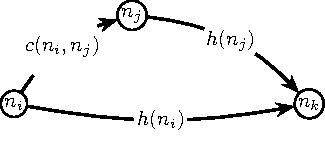
\includegraphics{disuguaglianza_consistenza.pdf}%
\end{figure}

La condizione di consistenza impone che i valori della funzione di valutazione $f$ dei nodi 
nell'albero di ricerca siano strettamente non-decrescenti all'allontanarsi dal nodo di 
partenza. Dati due nodi $n_j$, successore di $n_i$, se è soddisfatta si ha:
\begin{equation*}
    f(n_j)\geq f(n_i)
\end{equation*}
Dalla condizione di consistenza si aggiunge ad entrambi i membri $g(n_j)=g(n_i)+c(n_i,n_j)$:
\begin{gather*}
    h(n_j)\geq h(n_i)-c(n_i,n_j)\\
    h(n_j)+g(n_j)\geq h(n_i)-c(n_i,n_j)+g(n_j)=h(n_i)-\cancel{c(n_i,n_j)}+g(n_i)+\cancel{c(n_i,n_j)}\\
    f(n_j)\geq f(n_i)\tageq
\end{gather*}

Per cui spesso la condizione di consistenza sulla funzione euristica $h$ viene chiamata 
condizione monotona su $f$. 

\'{E} dimostrabile che se una funzione euristica $h$ è consistente allora è anche ammissibile. 

Se la condizione di consistenza è soddisfatta su $h$, allora quando l'algoritmo A* espande un nodo 
$n$ ha già trovato il percorso ottimo per $n$. In questo modo la ricerca su grafo non è 
differente dalla ricerca su un albero per quanto riguarda l'ottimalità della soluzione. 


\subsection{Algoritmo di Ricerca Locale: Hill-Climbing}


Nei problemi precedenti quando l'algoritmo risolutivo raggiungeva uno stato obiettivo, il cammino verso quello stato rappresenta una soluzione 
del problema. Tuttavia in alcuni problemi lo stato obiettivo contiene tutte le informazioni rilevanti per la soluzione, dove il cammino è 
irrilevante. Come esempio si consideri il problema dell otto regine, è indifferente il cammino attraverso gli stadi intermedi, solamente lo 
stato finale, la disposizione delle regine nello stato finale. 

Algoritmi di ricerca locale si utilizzano per risolvere questo tipi di problemi. In questi problemi è sempre presente uno spazio degli stati 
ed uno spazio degli stati aventi ciascuno una sua valutazione. Si può immaginare questi stadi su una superficie del territorio, uno spazio dove l'altezza 
di questo stato rappresenta la sua valutazione. L'algoritmo quindi itera su ognuno di questi stati per cercare quello di altezza maggiore, o minore, identificando 
quindi la soluzione al problema, indipendentemente dal cammino preso per raggiungerla. Questi punti di massimo rappresentano dei picchi, i cui punti adiacenti sono 
strettamente minori dello stato di massimo. Quindi l'algoritmo che parte da uno stato iniziale deve cercare un massimo globale in questo spazio, determinando quale sia 
tra i vari massimi locali ed i massimi locali piatto, e le ``spalle'' massimi locali ``piatti'', prima di un massimo globale:

\begin{figure}[H]%
    \centering%
    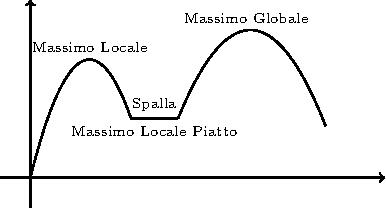
\includegraphics[scale=1.25]{grafico_massimi.pdf}%
\end{figure}

Questi algoritmi chiamati anche di miglioramento iterativo, si muovono sulla superficie cercando questi picchi, senza tenere traccia del cammino effettuato, tenendo 
solamente traccia dello stato attuale e dei suoi vicini o successori, gli stati immediatamente adiacenti. 
Bisogna formulare il problema in modo che l'algoritmo non rimanga bloccato tra due massimi locali. 

Questo algoritmo segue sempre le colline più ripide, si muove sempre verso l'alto nella direzione dei valori crescenti, e termina quando raggiunge uno stato per il quale 
si ha un picco che non ha vicino stati di valore maggiore. Tuttavia questo algoritmo può rimanere intrappolato su massimi locali. 

Non viene memorizzato lo stato corrente, solamente il valore attraverso nodi che contengono lo stato ed il suo valore. 

Esistono diversi tipi di algoritmi di questo genere per evitare di rimanere bloccati su picchi locali, utilizzando diverse tecniche. 
\begin{itemize}
    \item Steepest Ascent Hill-Climbing;
    \item First-Choice Hill-Climbing;
    \item Random-Restart Hill-Climbing (Iterated Hill-Climbing);
    \item Stochastic Hill-Climbing. 
\end{itemize}

\subsubsection{Algoritmo Steepest Ascent Hill-Climbing}

Si considera il seguente pseudocodice dell'algoritmo Hill-Climbing di tipo ``Steepest Ascent'':

\begin{minted}[escapeinside=||]{c}
    function |\textcolor{red}{HILL-CLIMBING}|(problem) returns a state local max

    current <- |\textcolor{magenta}{MAKE-NODE}|(|\textcolor{magenta}{INITIAL-STATE}|(problem))
    loop do 
        next <- |\textcolor{magenta}{MAX}|(|\textcolor{magenta}{EXPAND}|(current))
        if |\textcolor{magenta}{VALUE}|(next) < |\textcolor{magenta}{VALUE}|(current) then return |\textcolor{magenta}{STATE}|(current)
        current <- next
    end
\end{minted}

Dallo stato corrente si ricava il suo valore, in seguito comincia un ciclo che prende in considerazione tutti i successori e si sceglie come \verb|next| il nodo di 
valore più alto. Se tutti i nodi adiacenti hanno un valore minore di \verb|next| allora questo rappresenta la soluzione dell'algoritmo e l'algoritmo termina, tuttavia 
questo stato potrebbe corrispondere ad un massimo locale, invece se esiste uno stato adiacente di valore maggiore, questo diventa \verb|next| e si passa alla nuova 
iterazione. 

\subsubsection{Algoritmo Random-Restart-Hill Climbing}

L'algoritmo contiene una componente di ripartenza casuale, questo infatti conduce una serie di ricerche di Hill-Climbing partendo da stati generati casualmente. Questo 
algoritmo da un punto di vista teorico è completo, poiché con una serie infinita di ripartenze, sicuramente l'algoritmo visita tutti gli stati del sistema, trovando sicuramente 
la soluzione ottima del problema. 

\begin{minted}[escapeinside=||]{c}
    function |\textcolor{red}{RANDOM-RESTART-HILL-CLIMBING}|(problem) returns a state solution

    t <- 0
    best <- |\textcolor{magenta}{MAKE-NODE}|(NULL)

    repeat
        local <- false
        current <- |\textcolor{magenta}{RANDOM}|(problem)
        repeat 
            next <- |\textcolor{magenta}{MAX}|(|\textcolor{magenta}{EXPAND}|(current))
            if |\textcolor{magenta}{VALUE}|(next) > |\textcolor{magenta}{VALUE}|(current)
                then current <- next
            else local <- true
        until local
        t <- t + 1
        if |\textcolor{magenta}{VALUE}|(current) > |\textcolor{magenta}{VALUE}|(best)   
            then best <- current
    until t = MAX
    return |\textcolor{magenta}{STATE}|(best)
    end
\end{minted}

Il ciclo interno ad ogni iterazione genera un ottimo locale, e prova ad evitare ottimi locali effettuando una nuova ricerca da un nuovo stato scelto 
casualmente. L'algoritmo è completo con probabilità tendente ad uno, poiché è possibile generi come stato 
iniziale uno stato obiettivo. 

\subsubsection{Algoritmo Stochastic Hill-Climbing}

L'algoritmo Stochastic Hill-Climbing si ottiene modificando la procedura normale dell'algoritmo. Invece di valutare tutti i vicini dallo stato corrente, l'algoritmo 
sceglie casualmente uno solo dei suoi successori da valutare per determinare se si tratta il successore, ed in caso diventa il nuovo stato corrente \verb|next|, questo 
viene accetta con una probabilità che dipende dalla differenza della valutazione tra i due punti: $\Delta E=$\verb|VALUE(current)-VALUE(next)|. 

\begin{minted}[mathescape, escapeinside=||]{c}
    function |\textcolor{red}{STOCHASTIC-HILL-CLIMBING}|(problem) returns a state solution

    t <- 0
    current <- |\textcolor{magenta}{RANDOM}|(problem)
    best <- |\textcolor{magenta}{MAKE-NODE}|(NULL)

    repeat
        next <- |\textcolor{magenta}{RANDOM}|(|\textcolor{magenta}{EXPAND}|(current))
        if |$p=1/(1+e^{\Delta E/T})$| 
            then current <- next
            if |\textcolor{magenta}{VALUE}|(current) > |\textcolor{magenta}{VALUE}|(best)   
                then best <- current
        t <- t + 1
    until t = MAX
    return |\textcolor{magenta}{STATE}|(best)
    end
\end{minted}



Il nuovo stato viene scelto con una probabilità $p$, calcolata come:
\begin{equation}
    p=\displaystyle\frac{1}{1+e^{\Delta E/T}}
\end{equation}

In seguito dopo una serie di iterazioni l'algoritmo restituisce uno stato ottimo. L'algoritmo ha quindi un solo ciclo, e può scegliere un nuovo punto con una probabilità 
$p$, quindi anche di valore minore. Questa probabilità dipende da un parametro $T$ costante durante l'esecuzione dell'algoritmo. Se vale 1, la probabilità di 
accettazione è sostanzialmente pari al 100\%. 

%% TODO tabella / andamento rispetto a T di p

All'aumentare del valore i $T$ la probabilità di accettazione tende al 50\%, diventa quindi sempre meno importante la differenza della valutazione tra i due punti, 
effettivamente comporta una ricerca casuale, mentre al diminuire di $T$, la procedura rappresenta un semplice algoritmo Hill-Climbing. 

In caso di stati di valore uguale, la probabilità è del 50\%, se il valore dello stato \verb|next| è minore, la probabilità diminuisce, mentre se il valore di \verb|next| 
è maggiore dello stato corrente, la probabilità aumenta. 

%% TODO tabella / andamento rispetto a $\Delta E$

Bisogna trovare una ``link function'' tra l'intervallo $\Delta E/T$ e la probabilità $p$. 

%% TODO img andamento link function

La caratteristica di poter scegliere come passo uno stato peggiore questo algoritmo potrebbe evitare massimi locali. 

\subsubsection{Algoritmo di Simulated Annealing}

L'algoritmo di Simulated Annealing, introdotto nel 1983 da S. Kirkpatrick, C.D. Gelatt, Jr. e M.P. Vecchi nella rivista Science, è un algoritmo che migliora 
considerevolmente l'approccio dell'algoritmo precedente. Ha causato una vera e propria rivoluzione in termini di ottimizzazione, ebbe un enorme successo in ogni 
settore dell'informatica come l'algoritmo migliore per problemi di ricerca locale, anche solo nella sua versione base.  
Questo algoritmo è talmente importante che ogni anno vengono riuniti congressi annuali internazionali per discutere possibili ottimizzazioni. 


Questo algoritmo prende il nome dall'analogia con il processo di metallurgia per temprare un materiale, questo processo infatti raggiungere uno stato di struttura 
cristallina ad energia minima. La differenza principale con l'algoritmo stocastico, è la possibilità di variare il valore di $T$ diminuisce gradualmente durante l'esecuzione 
dell'algoritmo. Il valore di $T$ parte da un valore elevato, per poi diminuire nel tempo, come se fosse la temperatura durante un processo di temperatura, per cui l'algoritmo si 
comporta in modo molto simile ad un normale hill-climber. Inoltre sceglie sempre uno stato 
se è migliore del punto corrente. 

\begin{minted}[mathescape, escapeinside=||]{c}
    function |\textcolor{red}{SIMULATED-ANNEALING}|(problem) returns a state solution

    t <- 0
    current <- |\textcolor{magenta}{RANDOM}|(problem)
    best <- |\textcolor{magenta}{MAKE-NODE}|(NULL)

    repeat
        repeat
            next <- |\textcolor{magenta}{RANDOM}|(|\textcolor{magenta}{EXPAND}|(current))
            if |\textcolor{magenta}{VALUE}|(next) > |\textcolor{magenta}{VALUE}|(current) 
                then current <- next
                if |\textcolor{magenta}{VALUE}|(current) > |\textcolor{magenta}{VALUE}|(best)   
                    then best <- current
                else if |\textcolor{magenta}{RANDOM}\text{[}|0,1) < |$e^{-\Delta E/T}$| 
                    then current <- next
        until termination-condition
        T = g(T, t)
        t <- t + 1
    until halting-condition
    return |\textcolor{magenta}{STATE}|(best)
    end
\end{minted}

La probabilità di accettazione è leggermente diversa rispetto all'algoritmo precedente, poiché nel simulated annealing si considera solamente un semiasse dell'ascissa, dato che in caso \verb|next| sia migliore non viene calcolata la probabilità di accettazione. Si accetta sempre 
uno stato di valore migliore, mentre l'accettazione di uno stato peggiore dipende da una probabilità. 
Quindi il mapping della link function non viene realizzata sull'intero intervallo $(-\infty,+\infty)$, ma solo su metà dell'ascissa, su $[0,+\infty)$, per cui è 
sufficiente utilizzare la funzione $e^{-\Delta E/T}$ avente come dominio il semiasse $[0,+\infty)$ e come codominio $(0,1]$. 

Questo ciclo interno viene effettuato un certo numero di volte fino ad una condizione di 
terminazione, che verrà trattata nelle implementazioni future. 
Finito questo ciclo si abbassa leggermente la temperatura tramite una funzione $g$ e si incrementa il contatore 
delle iterazioni \verb|t|. 
Anche la condizione di terminazione dell'algoritmo dipende dallo specifico problema 
e verranno trattate in futuro. 


Molte implementazioni dell'algoritmo seguono la stessa sequenza di passi. Si assegna la variabile \verb|T| alla temperatura massima, e si sceglie uno stato corrente 
casuale al primo passo. Si determina un successore assegnandolo direttamente se è migliore oppure tramite la funzione di probabilità e si ripete per un certo numero di 
cicli, e come passo finale si diminuisce la temperatura e si ripete dal secondo passo se la temperatura non ha 
raggiunto la temperatura minima. Quando la temperatura ha raggiunto la temperatura minima, si può scegliere se terminare l'algoritmo o ripeterlo un certo numero di 
volte, ripartendo dal primo passo. 

\clearpage

\section{Linguaggio Python}

Python è un linguaggio di programmazione vastamente utilizzato nell'area dell'intelligenza artificiale e nel machine learning. Recentemente è diventato il linguaggio di 
programmazione più diffuso al mondo. Python è un linguaggio general-purpose, ideato da Guido van Rossum nel 1989, a più alto livello del C, poiché gestisce automaticamente le 
più fondamentali operazioni. Per cui è molto semplice e spesso utilizzato a fine didattico tra i primi linguaggi di programmazione insegnati. 

La versione di Python utilizzata nel corso è la versione 3, nell'ambiente Anaconda. Può essere avviato tramite un interprete. 

\subsection{Ambienti di Sviluppo}

I principali ambienti di programmazione di Python sono Anaconda, Eclipse e Google Colab. Tutte e 
tre permettono di programmare in modo semplificato. 
Esistono due approcci alla traduzione ed esecuzione dei programmi per i linguaggi di alto 
livello. Possono essere trasformati in un programma in linguaggio macchina ed eseguiti, 
compilazione, oppure ciascuna istruzione di alto livello può essere trasformata in almeno un'
istruzione di linguaggio macchina ed eseguita direttamente, interpretazione. 
Storicamente la modalità interpretata viene associata alla programmazione su linea di comando, 
e solamente su rari casi viene utilizzata, anche se con Python ha cominciato ad essere riutilizzata. 

Quindi non è presente una fase intermedia di compilazione o un programma compilato da 
eseguire, ma il programma viene eseguito direttamente istruzione per istruzione tramite un 
interprete. 
I linguaggi compilati sono specifici per ogni piattaforma, ma estremamente ottimizzati 
per quella esatta piattaforma. Mentre i linguaggi interpretati prevedono la 
distribuzione diretta del file sorgente, uguale per tutte le piattaforme, ma deve essere 
disponibile il programma interprete e sono generalmente più lenti poiché l'esecuzione attende 
ogni nuova istruzione da eseguire. 
In assenza di vincoli sul tempo dell'esecuzione il ritardo introdotto dall'interpretazione 
è accettabile. 

Linguaggi come C e C++ sono linguaggi compilati, mentre Python è un linguaggio interpretato. 
Java ha un approccio ibrido generando il bytecode, una versione di linguaggio macchina eseguibile 
dalla JVM, elaboratore virtuale simile ad un hardware tradizionale, con una conversione 
quasi uno ad uno delle istruzioni. 

Python è un linguaggio interpretata ad alto livello simbolico. Un programma Python può 
essere eseguito in modalità interattiva, dove ogni istruzione viene eseguita singolarmente, 
ed il suo output viene visualizzato sulla console in sequenza. Questo programma può essere 
interrotto, si possono rieseguire certe istruzioni, etc. Si può quindi modificare il flusso 
e le istruzioni sulla base dell'output ottenuto. Questo tipo di codice viene utilizzato 
per data analytics e exploration. 
Altrimenti all'interprete può essere passato l'intero programma come un file di estensione \verb|.py|. 
L'output viene visualizzato solamente se si invoca la funzione di stampa. 

Per utilizzare la modalità interattiva serve un ambiente di interazione, l'interprete 
più diffuso è Cpython. 

Può essere scaricato su tutte le piattaforme, aprendo una console si può entrare nella modalità interattiva con il comando \verb|python3|. 
Per uscire da questa modalità è sufficiente invocare la funzione \verb|quit()|. 

Anaconda è una distribuzione di Python che semplifica la gestione ed il deployment delle librerie. Permette di creare ambiente 
in cui installare versioni specifiche delle librerie compatibili con certi software. Il gestore di queste librerie o package 
si chiama conda e si usa principalmente da linea di comando e gestisce queste librerie e le mantiene aggiornate. Può essere 
installato insieme a Cpython. 

I principali comandi in Anaconda sono:
\begin{minted}{python}
    # crea un nuovo environment di versione specificata: 
    conda create -n nomeEnv python=versionePython 
    # visualizza la lista di environment creati:
    conda info -envs                 
    # attiva l'ambiente di sviluppo
    source activate nomeEnv            
    # installa il package specificato all'interno dell'ambiente corrente
    conda install nomePackage=versionePackage
\end{minted}
Se non viene specificata la versione, sia per Python che per i pacchetti da installare, 
conda utilizzerà l'ultima versione come default. 


Le principali librerie utilizzate in questo corso sono pandas, matplotlib, NumPy, SciPy, IPython e scikit-learn. 
Dentro Anaconda c'è un'interfaccia browser per avere un ambiente di programmazione per programmare chiamato Jupiter, dove è 
possibile attivare la linea di comando per programmare in modalità interattiva. Si può attivare con il comando \verb|jupiter notebook|, 
che mostra a schermo l'indirizzo a cui collegarsi per accedere, generalmente \verb|127.0.0.1|. Si analizzerà in seguito insieme 
all'ambiente Google Colab, anch'esso su un'interfaccia browser. 

Sui notebook è possibile inserire del testo, ed accetta macro e comandi in formato Markdown, e funzioni scritte in LaTeX. 

Eclipse è un ambiente di sviluppo storico, multi-linguaggio, installando dal marketplace il plugin pydev per poter programmare in 
Python. 

Google Colab è un ambiente di sviluppo fornito gratuitamente da Google, utilizzando risorse cloud, su di un singolo 
notebook, direttamente collegato all'account google. 
Ha un'interfaccia a blocchi interattiva, da data scientist, e permette di scegliere il runtime e la GPU da utilizzare per 
eseguire il programma. Il codice viene salvato su un notebook, quindi su un file di estensione \verb|.ipynb|, ed è possibile 
passare al Python tradizionale e viceversa. Su dispositivi mobile è possibile programmare con un'interfaccia molto simile ad un 
computer. 

Si divide il programma in celle per dividere il codice e permettere di elaborare singoli blocchi, senza dover ricalcolare 
tutti i blocchi già eseguiti. Questo inoltre rende il codice più chiaro e comprensibile. 

JupyterLab è un estensione di Jupyter che aggiunge funzionalità per programmare a progetto per visualizzare e gestire diverse 
tipologie di file. 


Si possono utilizzare anche ambienti virtuali come Docker per eseguire il codice su container isolati. 
Inoltre esistono ambienti dedicati all'ambito scientifico con un'analisi più dettagliata dei dati prodotti come spyder, ``The Scientific 
Python Development Environment''. 

\subsection{Operatori}

Alla creazione di una variabile non 
è necessario definirne il tipo, il nome identificativo è arbitrario e può contenere numeri, ma non cominciare con un numero, viene consigliato di utilizzare un carattere 
minuscolo come primo carattere del nome. Esistono 33 parole chiave, non utilizzabili come nomi di variabili. Si può assegnare un valore ad una variabile tramite l'operatore 
\verb|=|, senza specificarne il tipo. 

Esistono una serie di operatori aritmetici come \verb|+|, \verb|-|, \verb|*|, \verb|\|, \verb|**|, per l'elevamento a potenza, \verb|%| per il modulo. Una differenza 
tra Python 2 consiste nella gestione della divisione, infatti in Python 2 viene considerata solo la parte intera dell'operazione. Per ottenere lo stesso risultato 
esiste l'operatore \verb|\\|, chiamato ``floor division''. 

Gli operatori seguono un ordine di precedenza naturale, come la sintassi moderna matematica:
\begin{enumerate}
    \item Parentesi;
    \item Elevamento a potenza;
    \item Moltiplicazione e divisione;
    \item Addizione e sottrazione;
    \item Operatori con lo stesso ordine valutati da sinistra verso destra. 
\end{enumerate}

In Python sono presenti tutti gli operatori booleani del C come \verb|==| ed operatori di confronto come \verb|<, <=, >, >=|, in aggiunta sono presenti 
altri operatori \verb|is| ed \verb|is not|. Inoltre sono presenti due versione degli operatori logici \verb|&&| e \verb|and|, || e \verb|or| e \verb|!=| e \verb|not|. 
Come in C un qualsiasi valore diverso da zero corrisponde al booleano \verb|True|, inoltre associa numericamente questo valore ad 1, mentre \verb|False| a 0. \'{E} possibile convertire 
un tipo di dato booleano ad un tipo di dato numerico come un intero \verb|int| o un numero reale \verb|float|. 

Si possono inserire dati dall'utente tramite la funzione \verb|input()| e la funzione \verb|raw_input()| per lo stesso comportamento di Python 2, e si può convertire in un tipo 
specifico con \verb|tipo(var)|. I commenti vengono realizzati tramite il carattere \#. 

\subsection{Istruzioni Condizionali}

In Python per identificare funzioni o istruzioni condizionali non si usano parentesi, ma si indenta di quattro posizioni. Dopo la condizione dell'
istruzione condizionale vanno inserite dei due punti \verb|:|:
\begin{minted}{python}
    if condizione: 
        # corpo dell'if
    else:
        # corpo dell'else
\end{minted}


Si possono gestire le eccezioni con il costrutto \verb|try| ed \verb|except|:
\begin{minted}{python}
    try:
        # corpo del try
    except:
        # corpo dell'except
\end{minted}

\subsection{Funzioni Built-In, Moduli e Definizione di Funzioni}

In Python sono integrate tantissime funzioni utili, per svolgere attività comuni, utilizzabili senza doverle definire, queste sono funzioni ``built-in''. 
Per invocare funzioni presenti in un certo modulo e non built-in si utilizzata la notazione puntata \verb|nomeModulo.nomeFunzione()|. Alcune tra le funzioni 
built-in più utili sono \verb|max()| e \verb|min()| che restituiscono il carattere più grande e più piccolo in una stringa; la funzione \verb|len()| che restituisce 
la lunghezza della stringa. Per convertire variabili in certi tipi è già stata mostrata la funzione \verb|tipo()|, dove al posto di \verb|tipo| si inerisce il 
tipo specifico, si usa \verb|str| per convertire in una stringa. 

Per importare moduli contenenti altre funzioni si utilizza \verb|importa| seguito dal nome del modulo da scaricare, che crea un object module con quel nome, si può 
rinominare seguendo questa istruzione con \verb|as| seguito dall'alias del modulo. Si utilizza un alias per semplificare la notazione puntata. 


Dati gli algoritmi analizzati precedentemente, si nota la necessita di introdurre generatori di numero casuali. La maggior parte di generatori casuali, sono deterministici, 
ovvero dato lo stesso input, generano la stessa sequenza di numeri casuali. Si utilizzano quindi numeri pseudo-casuali, generati da un calcolo deterministico, ma non è quasi possibile 
distinguerli da numeri generati casualmente. In Python esiste il modulo \verb|random| contenente funzioni pertinenti alla generazione di numeri casuali. La 
funzione \verb|random()| genera un numero casuale tra 0.0, compreso e 1.0, non compreso. Un altra funzione \verb|randint()| accetta due parametri, estremi 
dell'intervallo, inclusi, per generare un numero intero tra loro compreso. Con la funzione \verb|choice()| si può scegliere un elemento casualmente da una sequenza 
passata come argomento. 

Per definire nuove funzioni si utilizza la parola chiave \verb|def|, specificando il nome, tra parentesi tonde gli argomenti ed i due punti, indentando di quattro posizioni 
per scrivere il corpo della funzione:
\begin{minted}{python}
    def nomeFunzione(listaArgomenti):
        # corpo della funzione
        # resto del codice
\end{minted}

Dopo aver passato degli argomenti ad una funzione, questi vengono assegnati a delle variabili locali. Si può utilizzare anche una variabile come argomento. Inoltre 
tutte le aggiunte possibili alle funzioni built-in, si possono effettuare sulle funzioni definite dall'utente. 

Si dividono le funzioni in due tipi ``fruitful function'', funzioni produttive, e ``void function'', funzioni vuote,  le prime restituiscono un valore, le seconde non restituiscono valore. Le prime quindi 
vengono usate per assegnare o inizializzare variabili. Se si tenta di assegnare il risultato di una void function ad una variabile, viene ottenuto un valore chiamato \verb|None|. 
Questo valore ha un suo proprio tipo. Per definire una funzione produttiva, nel corpo si inserisce la parola chiave \verb|return| seguita dai parametri da restituire come 
risultato della funzione. 

\subsection{Cicli}

Si possono realizzare cicli tramite il costrutto \verb|while| o \verb|for|, seguito da una condizione booleana e dai due punti \verb|:|:
\begin{minted}{python}
    while condizione: 
        # corpo del ciclo
\end{minted}

Si può interrompere il ciclo con \verb|break|, e si può saltare l'iterazione corrente con \verb|continue|. Quando bisogna iterare su una collezione, un insieme di elementi, 
si può realizzare un ciclo ``for-each'': 
\begin{minted}{python}
    for elemento in collezione: 
        # corpo del ciclo
\end{minted}

Se il valore dell'elemento non viene utilizzato all'interno del ciclo, ma solo per effettuare un numero definito di cicli, è convenzione utilizzare il carattere \verb|_| per distinguerlo:
\begin{minted}{python}
    for _ in collezione:
        # corpo del ciclo 
\end{minted}

\subsection{Stringhe}

Le stringhe sono sequenze di caratteri, indicizzati come fosse un array:
\begin{minted}{python}
    stringa[i] # (i+1)-esimo carattere
\end{minted}
La funzione già discussa \verb|len()| restituisce il numero di caratteri di una stringa, 
anche se può essere utilizzata per altri tipi di dati come dizionari. Poiché è strutturata come un array è possibile scandire ogni carattere della stringa individualmente 
con un ciclo for-each. 

Talvolta è comodo accedere ad una sottostringa, o ``slice'', della stringa di partenza. La selezione di una sottostringa è simile alla selezione di un carattere, 
utilizzando due indici divisi da due punti per indicare l'inizio e la fine della sottostringa, il primo estremo è compreso, mentre il secondo no:
\begin{minted}{python}
    stringa[i:j] # slice contenente i caratteri da i a j-1
\end{minted}

A volte si ha la necessità si realizzare una sottostringa che parte dall'inizio o la fine della stringa originaria, per effettuarlo si può omettere l'estremo 
corrispondente:
\begin{minted}{python}
    stringa[:j] # slice dall'inizio della stringa
    stringa[i:] # slice fino alla fine della stringa
\end{minted}

I valori di una stringa sono immutabili una volta definiti, per cui non è possibile modificarne il valore accedendo tramite indice, verrà sollevato un messaggio di errore. 
Si può modificare una stringa realizzando una nuova stringa, come variante, tramite l'operatore di concatenazione \verb|+|:
\begin{minted}{python}
    stringa = stringa_1 + stringa_2 
\end{minted}

L'operatore \verb|*| applicato su una lista, la replica un certo numero di volte specificato. 

L'operatore \verb|in| è estremamente importante, permette di individuare se una stringa è sottostringa di un'altra, restituisce un valore booleano vero o falso:
\begin{minted}{python}
    stringa_1 in stringa_2
\end{minted}

Si possono inoltre utilizzare operatori di confronto tra stringhe all'uguaglianza con \verb|==|, oppure con \verb|<, >|, per confrontarle in ordine alfabetico. 
In Python le maiuscole vengono prima delle minuscole. 
Le stringhe sono degli oggetti che oltre alla sequenza di caratteri contengono oltre i dati anche i metodi disponibili per ogni istanza dell'oggetto stringa. 

Con la funzione \verb|type| si ha la possibilità di identificare il tipo dell'oggetto su cui viene operata e \verb|dir| mostra i metodi disponibili. 
Per utilizzare un metodo si utilizza la notazione puntata con il nome dell'istanza dell'oggetto. 
Uno dei metodi sulle stringhe è \verb|find()| che prende come argomento una sottostringa, ed un indice opzionale da cui cercare il carattere, e restituisce la prima 
posizione dell'occorrenza della sottostringa specificata. 

Il metodo \verb|strip()| rimuove lo spazio bianco prima e dopo la stringa. Il metodo \verb|startswith()| restituisce un valore booleano se la stringa comincia 
con la sottostringa passata come argomento. Il metodo \verb|capitalize()| consente di impostare a maiuscolo il primo carattere, per mettere tutti i caratteri in 
maiuscolo si utilizza il metodo \verb|upper()|. 

L'operatore ``format'' \verb|%| permette di costruire stringhe formattando la stringa rispetto a dati contenuti in altre variabili. All'interno di una stringa 
chiamata ``format string'' si può inserire questo operatore seguito da una lettera per specificare il tipo di dato associato, chiamate ``format sequences''. Questa 
viene utilizzata come il primo argomento, mentre il secondo operando è la variabile da formattare, questo produce una stringa:
\begin{minted}{python}
    >>> x = 1
    >>> 'il numero è %d' % x
    'il numero è 1' 
\end{minted}

Se in una stringa compare una sequenza di format sequences si specifica l'operando come una sequenza, una tupla, tra parentesi tonde, separando gli elementi con virgole:
\begin{minted}{python}
    >>> x = 1
    >>> 'il %s è %d' % ('numero', x)
    'il numero è 1' 
\end{minted}
La tupla deve corrispondere in numero, ordine e tipo alle format sequences nella stringa. 
Si utilizza \verb|%d| per numeri interi \verb|%g| per floating point e \verb|%s| per stringhe. Utilizzando numeri è possibile specificare il numero di cifre significative da utilizzare per 
rappresentare il numero, inserendo un numero subito dopo l'operatore format. 

Esiste un nuovo operatore format, scrivendo tra parentesi graffe \verb|:| seguito dal carattere corrispondente al tipo, dopo la stringa si invoca il metodo \verb|format()| 
specificando nell'argomento il valore da inserire:
\begin{minted}{python}
    >>> 'il {:s} è {:d}' .format('numero', 1)
    'il numero è 1' 
\end{minted}
Questa implementa tutte le caratteristiche già trattate per il format \verb|%|. 

\subsection{Classi e oggetti}

La fonte di ispirazione della programmazione orientata agli oggetti è dovuta a lavori realizzati dalla comunità 
sull'intelligenza artificiale, nell'ambito della rappresentazione della conoscenza quando Marvin Minsky propose il 
formalismo dei frames nel 1975. Con tutte le caratteristiche dei moderni approcci di programmazione orientata agli 
oggetti. 

Questo paradigma di programmazione consiste nel mantenere i dati e le funzioni operabili su di essi vicine, raggruppate 
in entità chiamate oggetti. Una classe è una descrizione di un insieme di oggetti che hanno lo stesso comportamento, ed un 
oggetto è una singola istanza di questa classe, dove è definita anche un insieme di metodi da poter usare su questi oggetti. 

L'insieme di tutti i metodi resi disponibili da una classe, con la descrizione del loro comportamento, si chiama interfaccia 
pubblica della classe. 

Una classe in Python viene definita tramite la parola chiave \verb|class| seguita dal nome della classe, utilizzando 
la notazione dove ogni parola del nome ha la prima lettera maiuscola, ``Camel-case'':
\begin{minted}{python}
    class NomeClasse:
        pass 
\end{minted}

\verb|pass| è un placeholder ed indica dove sarà scritto codice, questa rappresenta una definizione di una classe minimale, 
definendo solamente il nome e nessun altro comportamento. 

Si può istanziare una nuova classe dato il suo nome: 
\begin{minted}{python}
    NomeClasse()
\end{minted}
Questo istanzia un oggetto appartenente alla classe specificata, allocata in una nuova zona di memoria, una variabile 
assegnata a questa nuova istanza mantiene il riferimento a questa zona di memoria, quindi si ha:
\begin{minted}{python}
    >>> a = NomeClasse()
    >>> b = NomeClasse()
    >>> a == b
    False
\end{minted}
Poiché quest'operazione di confronto effettuata sulle variabili ha azione sugli indirizzi di memoria contenuti. 
Le proprietà che una classe deve avere può essere definite utilizzando un metodo particolare costruttore chiamato \verb|.__init__()|. 
Questo inizializza una nuova istanza della classe ed assegna i valori al suo stato. Metodi con un doppio carattere \verb|_| 
vengono chiamati ``Dunder Methods'', per ``Data Underlined''. Al costruttore vengono passati i parametri che si vuole, ma 
è sempre necessario passare la variabile chiamata \verb|self| per definire nuovi attributi sull'oggetto. Poiché quando viene 
creata un'istanza di una classe, viene salvata automaticamente a questo parametro. 

\begin{minted}{python}
    class NomeClasse:
        def __init__(self, attributo1, ..., attributoN):
            self.attributo1 = attributo1
            # ...
            self.attributoN = attributo N
\end{minted}

Ognuna di queste assegnazioni in realtà crea anche un attributo chiamato con il nome utilizzato nella notazione puntata, riferita 
a \verb|self|, e contenente il valore assegnatoli dal parametro passato come input al costruttore. \verb|self| deve 
essere sempre il primo parametro. 

Gli attributi creati in questo modo vengono chiamati ``Istance Attributes'', attributi d'istanza, che sono attributi 
unici per ogni istanza della classe, chiamai al momento di costruzione dell'istanza. Ma possono essere definiti attributi 
comuni per tutte le classi, chiamati ``Class Attributes'', all'interno del corpo della classe, senza inserirli 
all'intero del costruttore:

\begin{minted}{python}
    class NomeClasse:
        attributo = 'valore' 
        def __init__(self, attributo1, ..., attributoN):
            self.attributo1 = attributo1
            # ...
            self.attributoN = attributo N
\end{minted}

Ogni istanza avrà gli stessi class attributes, contenenti gli stessi valori. Per istanziare una classe, avendo 
un costruttore, bisogna passare i parametri richiesti al momento di creazione:
\begin{minted}{python}
    >>> istanza = NomeClasse('valore1', ..., 'valoreN')
\end{minted}

Si passa un parametro in meno poiché \verb|self| viene gestito internamente, al momento della creazione dell'oggetto. Si 
può accedere ad un certo attributo sempre con la notazione puntata, e si può modificare. Si può modificare 
sia un attributo di classe o istanza. 

Gli istance methods sono funzioni definite all'interno di una classe, possono essere invocati da una qualsiasi istanza 
della classe. 

\'{E} buona norma utilizzare un metodo come \verb|description()| per fornire una stringa contenente informazioni utili per 
l'istanza della classe. Ma questo non è il modo migliore per ottenere. Si utilizza il metodo \verb|.__str__()| per 
restituire queste informazioni in formato di stringa:
\begin{minted}{python}
    class NomeClasse:
        attributo = 'valore' 
        
        def __init__(self, attributo1, ..., attributoN):
            self.attributo1 = attributo1
            # ...
            self.attributoN = attributo N
        
        def __str__():
            return f'{self.attributo1}, ..., {self.attributoN}'
\end{minted}

Quando viene invocata una funzione di stampa su un'istanza di questa classe, viene stampata la stringa definita da questo 
metodo:
\begin{minted}{python}
    >>> istanza = NomeClasse('valore1', ..., 'valoreN')
    >>> print(istanza)
    valore1, ..., valoreN
\end{minted}

%% TODO tutti i metodi con prefisso punto

\subsection{Collezioni}

\subsubsection{Liste}

Una lista è una sequenza di item di qualsiasi tipo, per cui a differenza di una stringa il tipo non è omogeneo. All'interno di una lista è possible 
inserire una lista, creando una lista annidata.  
Una lista si realizza specificando gli elementi tra parentesi quadre:
\begin{minted}{python}
    [item_1, item_2, [item_3, item_4]]
\end{minted}

Una lista che non contiene elementi si chiama lista vuota mediante \verb|[]|, oppure con il comando \verb|list()|. Si può assegnare ad una variabile una lista allo 
stesso modo di un valore:
\begin{minted}{python}
    >>> lista = [item_1, item_2, [item_3, item_4]]
\end{minted}

Le liste al contrario delle stringhe sono modificabili, con la stessa sintassi per le stringhe, specificando tra parentesi quadre l'indice corrispondente, ed è possibile 
aggiornare il valore contenuto in questo indice. Se ad un certo indice è presente una lista, questo elemento viene trattato come lista e quindi si possono utilizzare 
due coppie di parentesi quadre per indicizzare questi elementi annidati:
\begin{minted}{python}
    >>> lista[2][2]
    item_4
\end{minted}
Si può considerare una lista come un mapping tra indici ed elementi, come nelle stringhe possono essere variabili ed espressioni, se si prova a leggere o scrivere 
ad un indice non esistente si solleva un \verb|IndexError|. Mentre se si utilizza un indice negativo, si conta all'indietro partendo dalla fine della stringa. 
L'operatore \verb|in| ha un funzionamento analogo a quello per le stringhe. 

Un modo per scandire la lista è con un ciclo for-each, come per le stringhe, oppure iterando manualmente su ogni elemento. Questo si può effettuare tramite 
la funzione \verb|range()| che permette di iterare su un insieme di valori, fornito l'ultimo come argomento:
\begin{minted}{python}
    for i in range(len(lista)):
        # corpo del for
\end{minted}

L'operatore di concatenazione vale anche per le liste, analogamente per l'operatore \verb|*| che replica una lista un certo numero di volte. 
L'operatore slice può essere utilizzato anche sulle liste per ottenere una sottolista:
\begin{minted}{python}
    lista[i:j] # sottolista da i a j-1
    lista[:j]  # sottolista da 0 a j-1
    lista[i:]  # sottolista da i a len(lista)
    lista[:]   # copia della lista
\end{minted}
L'operatore slice può essere utilizzato per aggiornare una sequenza di elementi in una lista. La sottolista da aggiornare deve avere lo stesso numero dei valori della 
lista originaria. 

Come per le stringhe, le liste sono oggetti e contengono metodi built-in. 
Il metodo \verb|append()|. aggiunge un nuovo elemento alla fine di una lista, il metodo \verb|extend()| prende come argomento una lista e la concatena alla lista su cui 
si è operato. Se si passa una lista al metodo \verb|append()| si genera una lista annidata. 
Si può ordinare gli elementi di una lista dal minore al maggiore con \verb|sort()| in ordine alfabetico. Molti dei metodi su liste, come questi, sono metodi void. 

Per estrarre un elemento dalla lista si utilizza il metodo \verb|pop()| che estrae dalla lista l'ultimo elemento, oppure l'elemento di indice specificato, 
lo restituisce rimuovendolo dalla lista:
\begin{minted}{python}
    >>> lista.pop(1)
    item_2
    >>> print(lista)
    [item_1, [item_3, item_4]]
\end{minted}
L'operatore \verb|del| rimuove un elemento dalla lista:
\begin{minted}{python}
    >>> del lista[1]
    >>> print(lista)
    [item_1, [item_3, item_4]]
\end{minted}
Utilizzando lo slice si può rimuovere una sottostringa allo stesso modo:
\begin{minted}{python}
    >>> del lista[:1]
    >>> print(lista)
    [[item_3, item_4]]
\end{minted}

Se non si conosce l'indice dell'elemento da cancellare si può utilizzare il metodo \verb|remove()|, ma non restituisce alcun valore:
\begin{minted}{python}
    >>> lista.remove(item_2)
    >>> print(lista)
    [item_1, [item_3, item_4]]
\end{minted}

Alcuni metodi come \verb|sum()| possono essere invocati solamente se la lista contiene solo numeri, altri metodi possono essere invocati se la lista contiene dati 
confrontabili tra di loro. 
Si può convertire una stringa in una lista tramite la funzione \verb|list()|, suddividendo la stringa in caratteri singoli, mentre si può suddividere in parole singole, 
separate da spazi con la funzione \verb|split()|. Si può specificare un delimitatore in questa funzione \verb|split()| da utilizzare al posto del delimitatore di default 
spazio. La funzione inversa della \verb|split()| è il metodo \verb|join()|, permette di realizzare una stringa, applicato su una stringa contenente il delimitatore 
da utilizzare per separare gli elementi. Si può concatenare senza spazi con la stringa vuota \verb|[]|. 

In Python si possono confrontare due oggetti con l'operatore \verb|is|, se si creano due stringhe di contenuto uguale, Python realizza un unico oggetto stringa, 
mentre se vengono realizzare due liste, contenenti gli stessi elementi, sono due oggetti distinti.  
Le due liste sono equivalenti poiché hanno lo stesso valore, ma non sono identiche, poiché non sono lo stesso oggetto. Due oggetti identici sono anche equivalenti. 

Si può assegnare ad una variabile ad un'altra in modo che entrambe si riferiscano allo stesso oggetto, e quindi anche se si tratta di liste il confronto \verb|is| sarà 
verificato. Un oggetto che ha più di riferimenti ha un ``alias'', più di un nome, e si dice un oggetto ``aliased''. Se gli oggetti sono mutabili questo può essere 
fonte di errore. 
Si consiglia di evitare di utilizzare alias quando si lavora con liste ed oggetti mutabili. Si distingue tra operazioni che creano nuove liste ed operazioni che modificano 
lista, come l'operatore di concatenazione \verb|+| ed il metodo \verb|append()|, quest'ultimo modifica la lista su cui è invocato analogamente di \verb|extend()|, mentre l'operatore di 
concatenazione genera una nuova lista. 


C'è uno speciale costrutto per accedere a tutti gi elementi di una lista effettuando la stessa operazione su di loro e memorizzare i nuovi elementi in un'altra 
lista:
\begin{minted}{python}
    >>> lista_1 = [1, 2, 3]
    >>> lista_2 = [item * 2 for item in lista_1]
    >>> print(lista_2)
    [2, 4, 6]
\end{minted}

Quando bisogna accedere contemporaneamente a più liste si può utilizzare la sintassi che utilizza la parola chiave \verb|zip| per trattare la sequenza di liste 
passate contemporaneamente:
\begin{minted}{python}
    for item_1, item_2, ... in zip(lista_1, lista_2, ...):
        # corpo del ciclo, per ogni iterazione si ha
        # item_1 = lista_1[i], item_2 = lista_2[i], ...
\end{minted}
In questo modo si può iterare su tutte le liste insieme, senza dover specificare per ognuna il loro indice. Questa funziona associa le liste e termina alla lista più 
corta. 

\subsubsection{Dizionari e Set}

Un dizionario è simile ad una lista, ma più generale, permette di accedere agli elementi contenuti tramite una chiave definita 
a priori. Rappresenta un mapping tra due insiemi, uno di chiavi ed uno di valori, ogni chiave individua un valore, ogni item 
del dizionario è quindi una coppia tra una chiave ed un valore. 
Può essere costruito un dizionario vuoto tramite la funzione \verb|dict()|, e se stampato produce \verb|{}|. 
\begin{minted}{python}
    >>> str2num = dict()
    >>> print(str2num)
    {}
    >>>
\end{minted}

Per aggiungere un item nel dizionario, si utilizzano parentesi quadre per specificare la chiave e si assegna il suo valore contenuto, 
come se fosse l'indice di una lista:
\begin{minted}{python}
    >>> str2num['uno'] = 1
    >>> print(str2num)
    {'uno' : 1}
\end{minted}
Questo formato di output di un dizionario è un formato che può essere utilizzato per popolare un dizionario:
\begin{minted}{python}
    >>> str2num = {'uno' : 1, 'due' : 2, 'tre' : 3}
\end{minted}
Ma l'ordine in cui sono stati inseriti gli elementi non viene mantenuto, questo non costituisce un problema, poiché gli elementi non 
vengono identificati dalla loro posizione, ma attraverso una chiave. Se si prova ad accedere ad un elemento la cui chiave 
non esiste viene sollevato un errore. Per accedere ad un valore nel dizionario si utilizza la chiave come fosse un incide:
\begin{minted}{python}
    >>> str2num['uno']
    1
\end{minted}

Si può utilizzare la funzione \verb|len()| per determinare il numero di elementi in un dizionario e la parola chiave \verb|in| 
per determinare se una data chiave è presente in un dizionario, non controlla se è presente un valore:
\begin{minted}{python}
    >>> len(str2num)
    3
\end{minted}
Per visualizzare i valori si può utilizzare il metodo \verb|values()| che restituisce elementi su cui si può costruire una lista, su cui è possibile 
verificare la presenza di certi valori tramite \verb|in|. Questo operatore utilizza diversi algoritmi per le liste e per i 
dizionari, utilizza una ricerca lineare per le liste ed una tabella di hash per i dizionari. 



Una tupla è una sequenza di valori, simili ad una lista, di qualsiasi tipo, indicizzati da interi. Le tuple a differenza delle liste 
sono immutabili, ed è possibile confrontarle tra di loro, quindi è possibile siano utilizzate per realizzare chiavi di 
dizionari. 
Si definisce una tupla come una sequenza di valori divisi da virgole, ma convenzionalmente si tende ad includere questi valori 
in parentesi graffe per semplificare la leggibilità:
\begin{minted}{python}
    >>> t={1, 2, 3}
\end{minted}

Per creare una tupla con un unico valore, bisogna comunque inserire la prima virgola, altrimenti si creerebbe o una stringa o 
un dato di tipo uguale al tipo del primo elemento. 

Si può creare una tupla vuota con la funzione \verb|tuple()|, invece è possible inserire un argomento in questa funzione per 
generare una tupla dagli elementi della sequenza. Se si tratta di una stringa ogni carattere viene trattato come un 
elemento distinto, quindi viene scomposta. I vari operatori analizzati per le liste si possono utilizzare anche per le 
tuple:
\begin{minted}{python}
    t[i]        # valore all'indice i
    t[i:j]      # valori dall'indice i a j-1
    t[:j]       # valori dall'indice 0 a j-1
    t[i:]       # valori dall'indice i a len(t)
    t[:]        # copia della tupla
\end{minted}

Se si provasse a modificare un elemento verrebbe sollevato un errore, è comunque possibile creare una copia sostituendo solamente 
certi valori, così come per le stringhe, effettuando una concatenazione. 

Gli operatori di confronto funzionano sulle tuple e su altre sequenze su Python. Cominciano a confrontare dal primo elemento 
di ciascuna sequenza, se sono uguali passa all'elemento successivo fino a trovare una coppia di elementi diversi. Quindi gli 
elementi successivi non vengono presi in considerazione. 

Si può utilizzare la funzione \verb|sort()|, può essere utile con lo schema DSU, ``Decorate, Sort, Undecorate''. Secondo questo 
approccio si decora una sequenza costruendo un elenco di tuple con una o più chiavi di ordinamento che precedono gli elementi 
della sequenza, si ordina tramite questa funzione ed in seguito si rimuove questa decorazione estraendo gli elementi della 
sequenza. 

Una caratteristica di Python consente di assegnare più di una variabile alla volta, potendo inserire una 
tupla sul lato sinistro dell'assegnazione, senza parentesi tonde per convenzione. 
Un'applicazione interessante permette di scambiare i valori tra due variabili con una singola istruzione:
\begin{minted}{python}
    >>> a, b = b, a
\end{minted}

Il numero di valori a destra e sinistra dell'assegnazione devon corrispondere per non sollevare errori. 
Un altro metodo chiamato \verb|items()| permette di restituire una lista di tuple dove ogni tupla è una coppia 
chiave-valore. Questa lista non è ordinata, ma essendo le tuple comparabili, si può ordinare con il metodo \verb|sort()|. 


Gli insiemi sono collezioni non ordinate di altri oggetti. L'istruzione per creare un insieme è \verb|set()|, inserendo 
una sequenza di elementi. In un insieme non possono esserci elementi ripetuti quindi vengono rimossi 
al momento della creazione. 

Si possono effettuare le classi operazioni su insiemi, con metodi di unione \verb|union()|, 
intersezione \verb|intersection()|, differenza \verb|difference()| e differenza simmetrica \verb|symmetric_difference()|. 

\subsubsection{Liste Concatenate}
\label{sec:liste_concatenate}

Il tipo di dato astratto lista concatenata è diversa dal tipo di dato predefinito lista già presente su Python. Si parlerà di 
liste singolarmente concatenate. Questa lista è composta da un nodo, contenente il dato ed un puntatore all'elemento successivo 
di questa struttura concatenata. L'ultimo nodo della lista contiene un puntatore nullo. Per accedere agli elementi si hanno 
due puntatori di accesso, \verb|head| e \verb|tail|, per accedere in testa o in coda alla lista. 

\'{E} comodo avere un accesso facilitato a queste due posizioni per effettuare facilmente operazioni di aggiunta, rimozione, 
modifica in testa o in coda. Un nodo è una classe contenente questi due unici attributi:
\begin{minted}{python}
    class Node:
        data = ''
        next = None

        def __init__(self, data, next):
            self.data = data
            self.next = next
\end{minted}

L'utilizzo del paradigma orientato agli oggetti non è l'unico modo per definire una lista concatenata, ma è il modo 
utilizzato durante questo corso. 

Una lista concatenata è una classe contenente i riferimenti alla testa ed alla coda della lista, inizialmente 
assegnati al valore nullo, per generare una lista vuota:
\begin{minted}{python}
    class SinglyLinkedList:
        def __init__(self):
            self.__head = None
            self.__tail = None
\end{minted}

In realtà il campo dati è un riferimento ad un altro oggetto contenente i dati, ma per semplificare si considera il campo 
dati direttamente contenente questi. 

Per scandire la lista elemento per elemento si può utilizzare un puntatore ausiliario, inizialmente assegnato al 
primo elemento della lista:
\begin{minted}{python}
    p = self.__head
\end{minted}
Per passare all'elemento successivo bisogna assegnare questo puntatore al valore del puntatore a \verb|next| contenuto 
nel nodo corrente:
\begin{minted}{python}
    p = p.next
\end{minted}

Per scandire la lista quindi si utilizza un ciclo, fino a quando il valore contenuto in questo puntato \verb|p| non 
corrisponde al valore \verb|None|:
\begin{minted}{python}
    class SinglyLinkedList:
        def __init__(self):
            self.__head = None
            self.__tail = None

        def operazione():
            p = self.__head
            while p != None:
                # operazioni sul nodo
                p = p.next
\end{minted}

Per cominciare a scandire la lista da un punto preciso si può inserire un parametro di classe \verb|Node| a cui 
assegnare \verb|p|. Si vogliono realizzare i seguenti metodi sulle liste singolarmente concatenate:
\begin{itemize}
    \item \verb|append|: Inserimento in coda;
    \item \verb|insert_head|: Inserimento in testa;
    \item \verb|insert_position|: Inserimento in una posizione intermedia;
    \item \verb|delete|: Cancellazione di un elemento;
    \item \verb|is_empty|: Verifica se la lista è vuota. 
\end{itemize}

\begin{minted}{python}
    class SinglyLinkedList:
        def __init__(self):
            self.__head = None
            self.__tail = None

        def append(self, newNode)
            if self.__tail != None:
                self.__tail.next = NewNode
            if self.__head == None:
                self.__head = NewNode
            self.__tail = NewNode
            # newNode.next = None

        def insert_head(self, newNode):
            if self.__head == None:
                self.__tail = self._head
            newNode.next = self.__head
            self.__head = newNode

        def insert_position(self, newNode, position):
            p = self.__head
            i = 0
            while i < position - 1 and p != None:
                p = p.next
                i += 1
            newNode.next = p.next
            p.next = newNode

        def delete(self, position):
            if self.__head == None:
                return None
            if position == 0:
                self.__head = self._head.next
                return None
            p = self.__head
            i = 0
            while i < position - 1 and p.next != None:
                p = p.next
                i += 1
            if i != position - 1:
                return None
            p.next = p.next.next
            
        def is_empty(self):
            return self.__head == None
\end{minted}

\subsubsection{Liste Ordinate, Pile e Code}
\label{sec:lista_ordinata}

Una lista ordinata è una lista ai cui elementi sono ordinati rispetto ad una certa chiave. 
Ogni inserimento deve quindi rispettare l'ordine della lista. 

Questa lista si può implementare tramite la liste concatenate:
\begin{minted}{python}    
    class SortedLinkedList:
        def __init__(self):
            self.__head = None
            self.__tail = None
\end{minted}

Si suppone di poter effettuare un inserimento in posizione intermedia. Bisogna scandire la 
lista fino a quando il dato da inserire non è maggiore del dato contenuto nel nuovo nodo 
da inserire. Si considera la chiave e la lista ordinata in modo crescente:
\begin{minted}{python}
        def add(self, newNode)
            if self.__head == None or self.__head.data > newNode.data:
                self.insert_head(newNode)
            elif self.__tail.data < newNode.data:
                self.append(newNode)
            else: 
                p = self.__head
                while p.next != None and p.data < newNode.data:
                    p = p.next
                newNode.next = p.next
                p.next = newNode
\end{minted}

Una pila è un tipo di dato astratto basato sul modello delle liste che gestisce 
gli elementi, implementando la disciplina LIFO, ``Last-In, First-Out''. 
Le operazioni vengono effettuate su un estremo della lista chiamato testa \verb|top|. 

La classe \verb|Node| è sempre la stessa, viene definita con un attributo None 
inizializzato a \verb|None| e può essere comodo avere a disposizione una variabile che indica 
il numero di elementi nella pila:
\begin{minted}{python}
    class Stack:
        __top = None
        __size = 0
\end{minted}

Ogni inserimento in una pila è un inserimento in testa, si chiama ``push'':
\begin{minted}{python}
        def push(self, newNode):
            newNode.next = self.__top
            self.__top = newNode
            self.__size += 1
\end{minted}

Per effettuare un'estrazione si estrae un elemento dalla testa, e generalmente il dato 
estratto è di interesse:
\begin{minted}{python}
        def pop(self):
            p = self.__top
            if p != None
                self.__top = p.next
                p.next = None
            self.__size -= 1
            return p
\end{minted}

Le code sono un altro tipo di dato astratto che utilizzano il modello delle liste, ma 
applicano la disciplina FIFO, ``First-In, First-Out'':
\begin{minted}{python}
    class Queue:
        __head = None
        __tail = None
        __size = 0
\end{minted}

L'inserimento di un elemento avviene sempre in coda, e si chiama ``enqueue'':
\begin{minted}{python}
        def enqueue(self, newNode):
            if self.__head == None: 
                self.__head = mewNode
            else:            
                self.__tail.next = newNode
            self.__tail = newNode
            self.__size += 1 
\end{minted}

Per rimuovere il primo elemento, si utilizza la funzione ``dequeue'':
\begin{minted}{python}
        def dequeue(self):
            p = self.__head
            if p != None
                self.__head = p.next
                p.next = None
            self.__size -= 1
            return p
\end{minted}

\subsection{Implementazioni}

La tecnica della ``memoization'' permette di implementare in modo efficiente funzioni che 
necessitano di salvare o memorizzare gli stadi intermedi di un'operazione, come può essere 
una funzione che calcola il fattoriale o numeri di fibonacci. 

Utilizzando una lista si possono salvare i valori intermedi calcolati, senza doverli 
ricalcolare in iterazioni successive dell'algoritmo. 

Un'esempio di quest'implementazione è la seguente:
\begin{minted}{python}
    def fattoriale_ric(n):
        if n == 1:
            return [1]
        sequenza = fattoriale_ric(n-1)
        sequenza.append(sequenza[-1] * n)
        return sequenza    
\end{minted}
In questo modo si evitano alcune inefficienze come dover chiamare la funzione \verb|len()| ad 
ogni iterazione, essendo una funzione lineare, il costo totale sarebbe quadratico. Analogamente 
per il calcolo della sequenza di Fibonacci fino ad un certo indice:
\begin{minted}{python}
    def fibonacci_ric(n):
        if n == 0:
            return [0]
        elif n == 1:
            return [0, 1]
        sequenza = fibonacci_ric(n-1)
        sequenza.append(sequenza[-1] + sequenza[-2])
        return sequenza
\end{minted}
Per implementare in modo efficiente queste operazioni non bisogna ricominciare ad ogni 
iterazione l'operazione che si vuole ottenere. 

Queste operazioni possono essere implementate utilizzando la stessa tecnica anche con un 
approccio iterativo. 


Un modo efficiente per scambiare due porzioni di una lista, noto l'indice $i$ in cui termina la 
prima sotto-lista, consiste nell'utilizzo dell'operatore 
slice e della concatenazione delle due sottoliste:
\begin{minted}{python}
    lista = lista[i:] + lista[:i]
\end{minted}

\subsubsection{Funzioni Anonime}

In Python si possono assegnare ad una lista i nomi di alcune 
funzioni considerate, e si può accedere a queste tramite l'indice della lista, inserendo 
i parametri tra parentesi tonde come se fosse la funzione stessa:
\begin{minted}{python}
    lista_funzioni = [funzione1, ..., funzioneN]
    lista_funzioni[i](parametri)
\end{minted}

Ma questo richiede comunque di definire precedentemente delle funzioni. ALtrimenti è possibile 
inserire direttamente nell'assegnazione alla lista la loro definizione utilizzando la 
notazione lambda. Questo è un aspetto della programmazione funzionale, utilizzabile su Python 
tramite la parole chiave \verb|lambda|, specificando gli argomenti della funzione, e dopo \verb|:| 
si inserisce l'operazione che produce il risultato di questa funzione:
\begin{minted}{python}
    lambda parametri : # operazioni sui parametri per produrre un output
\end{minted}

Quindi una lista contenente funzioni anonime è del tipo:
\begin{minted}{python}
    lista_funzioni = [lambda parametri1 : operazioni1, ..., lambda parametriN: operazioniN]
\end{minted}

\subsubsection{Dynamic Programming}

Per determinare l'efficienza di un algoritmo, si può utilizzare il comando \verb|%time| per 
ottenere informazioni sul tempo di utilizzo del processore da parte della funzione:
\begin{minted}{python}
    >>> %time funzione(parametri)
\end{minted}


Il ``memoization'' è un approccio al ``dynamic programming'' che risolve questo problema in modo 
top down, scomponendo il problema in sotto-problemi, e salvando i risultati parziali in una 
tabella. Quando deve eseguire un nuovo sotto-problema, cerca prima se sono già presenti in questa 
tabella, prima di calcolare direttamente il risultato. 
Si può implementare il calcolo della sequenza di Fibonacci utilizzando questo approccio. Per 
determinare se è necessario calcolare direttamente il risultato parziale, si usa il costrutto 
try-except. In questo costrutto si prova ad accedere all'elemento, se questo accesso solleva 
un errore ovvero un fallimento, il programma calcolare direttamente questo valore parziale:

\begin{minted}{python}
    def fibonacci_memoization(n, m = None):
        if m == None:
            m = {}
        if n <= 1:
            return n
        try: 
            return m[n]
        except:
            risultato = fibonacci_memoization(n - 1, m) + fibonacci_memoization(n - 2, m)
            m[n] = risultato
            return risultato
\end{minted}

Si utilizza in questo caso si utilizza un risultato, popolando la tabella ad ogni iterazione $i$, 
inserendo il risultato parziale utilizzando come chiave questo stadio parziale $i$. 

Questo approccio è decisamente più veloce dell'implementazione precedente \verb|fibonacci_ric|, 
avendo una complessità temporale lineare $O(n)$. 

Invece di utilizzare il costrutto try-except si può utilizzare un'istruzione condizionale 
per verificare che il valore di chiave $i$ considerato è presente nel dizionario con 
l'operatore \verb|in|:
\begin{minted}{python}
    m = {}
    def fibonacci_memoization(n):
        if n <= 2:
            return 1
        if n not in m:
            m[n] = fibonacci_memoization(n-1) + fibonacci_memoization(n-2)
        return m[n]
\end{minted}

Oltre all'approccio di memoization si può utilizzare un metodo duale chiamato ``tabular'', 
con una disciplina bottom up, partendo dai sotto-problemi più piccoli e memorizzando i loro 
risultati parziali su una tabella, combinando queste soluzioni per risolvere i successivi 
problemi, memorizzando i loro risultati sulla stessa tabella. 

Si considera un'implementazione utilizzando questo approccio della sequenza di Fibonacci:
\begin{minted}{python}
    def fibonacci_tabular(n):
        tab = [0,1]
        for i in range(2, n+1):
            tab.append(tab[i-1] + tab[i-1])
        return tab[n]
\end{minted}

Anche questo approccio ha un'implementazione in tempo lineare $O(n)$. 

\subsubsection{Algoritmo Greedy: Problema di Ricerca di un Itinerario}

L'algoritmo ``Greedy'' è un algoritmo best-first, che utilizza conoscenza euristica per 
determinare il miglior nodo dalla frontiera da espandere. La conoscenza si rappresenta tramite 
una funzione di valutazione $f$, per ogni funzione di valutazione si possono definire diversi 
algoritmi di ricerca informata. Generalmente la frontiera viene realizzata come una sequenza 
ordinata di nodi, sulla abase di questa funzione $f$. 

Nell'algoritmo Greedy, la funzione di valutazione è la funzione euristica $h$, definita in 
base alla conoscenza sul dato problema per stimare la ``distanza'' dello stato corrente dalla soluzione. 

Per problemi di viaggio e della ricerca di itinerari, la distanza rappresenta la distanza fisica 
dallo stato corrente alla destinazione. Una delle funzioni utilizzate in questi problemi come 
euristica è la distanza in linea d'aria. 

Per implementare questo tipo di algoritmi di viaggio è necessario rappresentare lo spazio degli 
stati, generalmente ottenuto da una mappa, quindi come un grafo connesso. Si può realizzare 
come un dizionario, dove uno stato viene utilizzato come chiave e corrisponde ad un insieme 
dei suoi stati successori:
\begin{minted}{python}
    connections[stato] = {successore1, ... , successoreN}
\end{minted}

Non è l'unica possibilità per rappresentare un grafo, esistono infatti molte librerie 
realizzate unicamente per gestire grafi come questi, ma è utile ai fini didattici realizzare 
il problema per intero prima di avvalersi di librerie esterne. 
In questa rappresentazione del grafo non è presente la distanza tra le città, può essere inserita 
come un insieme di tuple contenenti lo stato successore e la distanza a quello stato. 
Ma per implementare l'algoritmo Greedy non è necessario sapere la distanza, poiché si utilizza 
solamente la funzione euristica, e non il percorso parziale, come nell'algoritmo A*. 
Per mettere in evidenza questo concetto viene intenzionalmente omessa in questa rappresentazione 
del grafo. 

Anche la funzione euristica $h$ viene implementata tramite un dizionario, contenente per ogni 
stato, utilizzato come chiave, il suo valore:
\begin{minted}{python}
    h[stato] = valore
\end{minted}

Per realizzare i nodi dell'albero di ricerca si crea una nuova classe, chiamata \verb|Node|, 
contenente lo stato, un riferimento 
al suo nodo genitore ed il valore della funzione euristica per lo stato contenuto:
\begin{minted}{python}
    class Node:
        def __init__(self, state, parent, h):
            self.state = state
            self.parent = parent
            self.h = h
\end{minted}

Ulteriormente si possono inserire la sua profondità nell'albero ed una lista dei suoi nodi figli, 
per rappresentare graficamente l'albero:
\begin{minted}{python}
    class Node:
        def __init__(self, state, parent, h):
            self.state = state
            self.parent = parent
            self.h = h
            self.child = []
            self.depth = 0
\end{minted}

Per rappresentare graficamente l'albero bisogna inserire inoltre un metodo per aggiungere 
dei figli al nodo:
\begin{minted}{python}
        def addChild(self, childNode):
            self.children.append(childNode)
            childNode.parent = self
            childNode.depth = self.depth + 1
\end{minted}

Inoltre per visualizzare il percorso quando viene individuata la soluzione, si definisce 
un altro metodo:
\begin{minted}{python}
        def printPath(self):
            if self.parent != None:
                self.parent.printPath()
            print("-> ", self.state.name)
\end{minted}

Questo metodo invocato su un nodo risale i nodi dell'albero fino ad arrivare alla radice, 
definite con un campo parent contenente \verb|None|, quindi comincia a stampare gli 
stati a partire dalla radice. 

Si definisce ulteriormente la classe \verb|State| per rappresentare gli stati del problema, con 
un campo nome per identificare gli stati. Questa classe ha i metodi per restituire lo 
stato iniziale, per restituire i successori di questo nodo, accedendo al dizionario delle 
connessione degli stati, e per controllare se è lo stato obiettivo:
\begin{minted}{python}
    class State:
        def __init__(self, name = None):
            if name == None:
                self.name = self.getInitialState()
            else:
                self.name = name

        def getInitialState(self):
            initialState = statoIniziale
            return initialState

        def successorFunction(self):
            return connections[self.name]

        def checkGoalState(self)
            return self.name == statoObiettivo
\end{minted}

Per implementare la frontiera si utilizza una lista ordinata con classi ed oggetti, ma esistono 
strutture dati più efficienti per implementare una ``priority queue'', come l'heap. Python 
contiene un'implementazione di una lista con priorità, ma analogamente allo spazio degli stati 
si utilizza per fini didattici un'implementazione dedicata:
\begin{minted}{python}
    class Item:
        value = None
        node = None
        next = None

        def __init__(self, value, node):
            self.value = value
            self.node = node
            self.next = None
\end{minted}

La classe della lista ordinata è la stessa definita precedentemente nella sezione 
dedicata \ref{sec:lista_ordinata}. 
Sono necessari i metodi di inserimento, mantenendo l'ordinamento, il metodo di 
estrazione del primo elemento \verb|remove_front|, analogo ad una \verb|pop| per le pile, 
ed un metodo per controllare se la frontiera è vuota \verb|is_empty()|. Questi metodi sono già stati descritti nella sezione specificata 
\ref{sec:liste_concatenate}. 


Si definisce quindi l'algoritmo Greedy, inizializzando la frontiera, lo stato iniziale e 
l'euristica. Inserendo la radice nella frontiera:
\begin{minted}{python}
    def Greedy_Best_First():
        fringe = SortedLinkedList() 

        initialState = State()
        
        root = Node(initialState, None, h[initialState.name])

        fringe.add(Item(root.h, root))
\end{minted}

In seguito bisogna inserire il ciclo che verrà eseguito fino all'esaurimento della frontiera, 
controllando ad ogni iterazione che non sia vuota tramite il metodo \verb|is_empty()|. 
Ad ogni iterazione viene estratto il primo nodo dalla frontiera e si controlla se questo è 
un nodo obiettivo. Se è un nodo obiettivo si interrompe l'esecuzione e viene stampato il 
percorso ottenuto. 
Altrimenti bisogna continuare l'esecuzione espandendo questo nodo, ed inserendo i suoi 
successori all'interno della frontiera:

\begin{minted}{python}
        while not fringe.is_empty():
            itemRemoved = fringe.remove_front()
            currentNode = itemRemoved.node

            if currentNode.state.checkGoalState():
                currentNode.printPath()
                break
            else: 
                childStates = currentNode.state.successorFunction()
                for childState in childStates:
                    childNode = Node(State(childState), currentNode, 
                                        h[State(childState).name])
                    # per rappresentare graficamente l'albero:
                    # currentNode.add(childNode) 
                    fringe.add(Item(childNode.h, childNode))
\end{minted}

Iterando su tutti gli stati successori del nodo corrente bisogna creare il nodo corrispondente 
ed aggiungere l'elemento relativo a questo nodo nella frontiera. 
Quest'implementazione utilizza un approccio tree-search. 

Se invece si utilizza la coda di priorità da una libreria esterna, bisogna importa, 
ed utilizzare i suoi metodi allo stesso modo della lista ordinata utilizzata 
precedentemente:
\begin{minted}{python}
    import queue as queue

    # per la creazione:
    fringe = Queue.PriorityQueue()

    # per l'inserimento si utilizza una tupla, (euristica, nodo):
    fringe.put((node.h, node))

    # per la verifica della frontiera vuota:
    fringe.empty()

    # per la rimozione del primo elemento:
    fringe.get()
\end{minted}

\subsubsection{Algoritmo A*: Problema di Ricerca di un Itinerario}

L'algoritmo A* è un algoritmo Best-First, ma è molto migliore rispetto all'algoritmo Greedy 
poiché la sua funzione di valutazione considera anche il percorso parziale dalla 
radice al nodo corrente. Si può implementare nelle due versioni dell'algoritmo Best First, 
in modalità Tree-Search e Graph-Search rispettivamente. 
Nella modalità Tree-Search ogni volta che viene espanso uno stato, i nodi corrispondenti 
ai suoi stati successori vengono inseriti nella frontiera, mentre nella Graph-Search gli 
stati già visitati vengono inseriti in un insieme, per non ripetere nuovamente lo stesso 
stato. Questo viene effettuato senza inserire gli stati già presenti in questo insieme 
in frontiera. 

In questa implementazione è necessario conoscere la distanza parziale, quindi lo spazio 
degli stati viene realizzato tramite un dizionario, dove i valori sono costituiti da coppie 
stato successore e distanza:
\begin{minted}{python}
    connections[stato] = {[successore1, distanza1], ..., [successoreN, distanzaN]}
\end{minted}

La funzione euristica viene definita allo stesso modo dell'algoritmo precedente, 
tramite un dizionario:
\begin{minted}{python}
    h[stato] = valore
\end{minted}

Si definisce la classe di un nodo, che ora deve contenere anche la distanza parziale:
\begin{minted}{python}
    class Node:
        def __init__(self, state, parent, f, partialPath):
            self.state = state
            self.parent = parent
            self.f = f
            self.partialPath = partialPath
            # self.child = []
            # self.depth = 0
\end{minted}

I metodi per stampare il percorso sono gli stessi dell'algoritmo Greedy, così come la 
classe che definisce uno stato del problema e la lista ordinata per la frontiera.

Si implementa direttamente la versione Graph-Search dell'algoritmo. Si inizializza allo 
stesso modo dell'implementazione precedente, ma bisogna inizializzare un'altra collezione 
per rappresentare l'insieme dei nodi già visitati:
\begin{minted}{python}
    def A_Star():
        fringe = SortedLinkedList() 
        close = []

        initialState = State()
        root = Node(initialState, None, h[initialState.name], 0)

        fringe.add(Item(root.f, root))
\end{minted}

Analogamente la prima parte dell'algoritmo dentro al ciclo è uguale, bisogna estrarre un nodo 
dalla frontiera, controllare se corrisponde allo stato obiettivo ed in caso stampare 
la soluzione ottenuto e terminare l'esecuzione dell'algoritmo:
\begin{minted}{python}
    while not fringe.is_empty():
            itemRemoved = fringe.remove_front()
            currentNode = itemRemoved.node

            if currentNode.state.checkGoalState():
                currentNode.printPath()
                break
\end{minted}
Altrimenti bisogna verificare se non è già stato espanso, in caso si aggiunge alla lista dei 
nodi già visitati e si espande, iterando sui suoi stati figli per creare i corrispondenti 
nodi ed aggiungerli alla frontiera, se non sono già stati visitati:
\begin{minted}{python}
            if currentNode.state.name not in close:
                close.append(currentNode.state.name)

                childStates = currentNode.state.successorFunction()
                for (childState, distance) in childStates:
                    g = childState.partialPath + distance
                    f = g + h[childState]
                    childNode = (childState, currentChild, f, g)

                    if childState.name not in close:
                        fringe.add(Item(childNode.f, childNode))
\end{minted}
Questo controllo non è necessario, poiché se viene estratto un nodo corrispondente ad un elemento 
già espanso, non viene comunque espanso. 

\subsubsection{Algoritmo Hill-Climbing: Problema di Ricerca di una Stringa}

Si considera la versione First-Choice dell'algoritmo Hill-Climbing. L'algoritmo dato uno stato corrente sceglie un valore migliore, in base alla versione dell'algoritmo, fino a quando 
non trova un massimo locale. Questo algoritmo quindi passa tra stati di valore sempre crescente e termina quando raggiunge il picco. 
In questa versione First-Choice, l'algoritmo sceglie casualmente uno stato adiacente e verifica se questo stato è il migliore, ed in caso lo considera il nuovo stato corrente. 
Si vuole applicare questo problema dove da una stringa iniziale di $n$ caratteri si vuole raggiungere una stringa obiettivo di $n$ caratteri. 
Bisogna individuare gli stati e gli operatori da poter applicare ad una stringa. Uno stato è un'istanza di una stringa da $n$ caratteri, ed un operatore può modificare un singolo di questi 
$n$ caratteri sostituendolo con uno dei caratteri disponibili. In questo modo vengono creati gli stati adiacenti del problema. 
Per considerare tutti i successori bisognerebbe considerare per ciascuno degli $n$ caratteri uno dei caratteri disponibili. 

La funzione di valutazione in questo problema è la distanza dalla stringa obiettivo, calcolabile come la somma delle distanze dei singoli caratteri dalla stringa corrente alla stringa obiettivo. 

I caratteri disponibili sono i $100$ caratteri stampabili su Python, visualizzabili con \verb|.printable|, dopo aver importato l'opportuno modulo \verb|string|. Il numero di stati possibili è $100^n$, 
mentre per ognuna delle $n$ posizioni si hanno $100$ posizioni diverse, quindi dato uno stato si hanno $100\cdot n$ stati adiacenti. 

Per generare uno stato iniziale, si può generare una stringa di $n$ caratteri scelti casualmente:
\begin{minted}{python}
    import random
    import string
    
    def generate_random_string(length):
        return [random.choice(string.printable) for _ in range(length)]
\end{minted}

Per calcolare la distanza tra due stringhe si può utilizzare la funzione built-in \verb|ord()| che restituisce il codice Unicode del carattere inserito come parametro. Si può iterare su ognuno di questi caratteri 
e calcolarne la distanza dalla stringa obiettivo:
\begin{minted}{python}
    def evaluate(sol):
        trg = list(targetString)
        diff = 0
        for i in range(len(trg)):
            diff += abs(ord(sol[i]) - ord(trg[i]))
        return diff
\end{minted}


Per scegliere il successore bisogna scegliere casualmente la posizioni da modificare ed il carattere da sostituire:
\begin{minted}{python}
    def tweak(sol):
        i = random.randint(0, len(sol) - 1)
        sol[i] = random.choice(string.printable)
\end{minted}

L'algoritmo quindi itera continuamente fino a quando lo stato corrente non è nullo, visitando sempre e solo stati di valore minore di quello corrente. Dato che gli algoritmi Hill-Climbing risolvono sia problemi di 
massimo che di minimo, essendo tra loro duali. Si può scegliere se farlo partire da una stringa casuale oppure da stringa specificata dall'utente. 
\begin{minted}{python}
    def First_Choice_Hill_Climbing(initialString):
        currentState = initialString
        # currentState = generate_random_string(length)
        currentEval = evaluate(initialString)

        while True:
            if currentEval == 0:
                break
            
            nextState = tweak(list(currentState))
            nextEval = evaluate(nextState)

            if nextEval < currentEval:
                currentState = nextState
                currentEval  = nextEval
\end{minted}

Questi algoritmi operano nel discreto, anche se molte volte si lavora su domini continui, e sono necessari altri controlli e test diversi per poter implementare algoritmi di ricerca. 

\subsubsection{Algoritmo Simulated Annealing: Problema delle n Regine}

In questo algoritmo si parte da uno stato iniziale casuale e si sceglie casualmente un successore, come nell'algoritmo precedente, e si accettano sempre stati adiacenti migliori, mentre in base ad una probabilità 
se peggiori. Una variabile chiamata temperatura determina il cambiamento di questa probabilità. All'aumentare della temperatura diventa sempre meno probabile che stati adiacenti di valore peggiore vengono 
scelti dall'algoritmo. Questo algoritmo termina quando trova uno stato obiettivo, oppure se rispetta cerca condizioni di terminazione. 

Il problema delle $n$ regine consiste nell'individuare una disposizione su una scacchiera $n\times n$, dove $n$ regine presenti non si attaccano fra di loro. Ovvero se si potessero muovere non potrebbero 
catturarsi a vicenda. Una regina negli scacchi si può muovere sia verticalmente, che orizzontalmente, che diagonalmente. 
In questo problema lo spazio degli stati consiste in stati contenenti $n$ regine, una in ogni colonna ed una in ogni riga. In questo modo bisogna solamente analizzare conflitti sulle diagonali. In questo modo 
viene limitata notevolmente lo spazio degli stati e viene semplificata la sua rappresentazione, invece che con una matrice, con un semplice vettore. 
Dato uno stato per considerare i successori si considera uno scambio tra due colonne, per mantenere il primo vincolo sugli stati. 
Lo stato obiettivo è un qualsiasi stato dove le regine non sono in conflitto tra di loro. La funzione di valutazione sono il numero di attacchi in una data disposizione della scacchiera, che si vuole 
minimizzare. 
Una scacchiera si può rappresentare come un vettore lungo $n$, dove l'indice individua la colonna, ed il valore contenuto la riga corrispondente, poiché una sola regina può essere su ogni colonna ed ogni riga. 
Per passare da uno stato ad uno adiacente si utilizza una funzione \verb|tweak()|. Questa funzione scambia due colonne, scegliendo casualmente due indici ed invertendo i loro valori:
\begin{minted}{python}
    def tweak(sol):
        solCopy = np.copy(sol)

        x = random.randint(0, n-1)
        y = random.randint(0, n-1)
        while x == y:
            y = random.randint(0, n-1)
        solCopy[x], solCopy[y] = solCopy[y], solCopy[x]

        return solCopy
\end{minted}

Per inizializzare il problema si sceglie casualmente uno stato iniziale. Quindi partendo da uno stato iniziale, come potrebbe essere una disposizione avente le regine sulla diagonale principale, ed operare 
un certo numero di volte la funzione \verb|tweak()| per ottenere uno stato casuale:
\begin{minted}{python}
    def initialize(sol):
        for _ in range(0, initialSteps):
            sol = tweak(sol)
        return sol
\end{minted}

Questo valore \verb|initialSteps| deve essere un numero significativo per realizzare ad ogni esecuzione uno stato nuovo casuale. 
Convenzionalmente la funzione di valutazione nel Simulated-Annealing viene chiamata energia, poiché in metallurgia per effettuare questo processo si vuole appunto minimizzare l'energia del sistema. 
La funzione di valutazione deve considerare solamente gli spostamenti in diagonale delle regine sulla scacchiera. Queste si possono spostare in quattro possibili direzioni: $(1,1)$, $(1,-1)$, $(-1, 1)$ e $(-1,-1)$. 
Ovvero possono incrementare o decrementare gli indici di riga o colonna di uno. Per verificare se sono presenti conflitti, data la posizione originale di una regina, si segue una delle diagonali individuata da 
una di queste quattro direzioni, fino a raggiungere il bordo della scacchiera. Si può implementare realizzando la scacchiera tramite una matrice contenente solo valori nulli, ed inserendo le regine 
con un valore specifico. In questo modo ci si può spostare sulle diagonali come su un piano cartesiano discreto, su direzioni individuate da spostamenti unitari d$x$ e d$y$. Iterando su ogni regina, si 
considera la sua posizione corrente $x$ e $y$, e si incrementa progressivamente tramite questi spostamenti unitari su una delle diagonali. Ad ogni passo si controlla se la posizione è interna alla scacchiera, 
ed in caso si termina la ricerca per questa diagonale, oppure se la casella corrispondente contiene una regina, ed in caso si incrementa il contatore dei conflitti. Questa ricerca dei conflitti termina dopo 
aver percorso le diagonali di tutte le regine contenute nello stato passato come parametro, restituendo il numero di conflitti ottenuti. Questo numero sarà sempre pari, poiché per ogni coppia di regine in conflitto 
sono possibili due attacchi sia dalla prima che dalla seconda regina. 
\begin{minted}{python}
    def energy(sol):
        board = [[0] * n for i in range(n)]
        for i in range(0, n):
            board[sol[i]][i] = 1
        
        dx = [1, 1, -1, -1]
        dy = [1, -1, 1, -1]

        conf = 0
        for i in range(0, n):
            x = sol[i]
            y = i
            for j in range(0, 4):
                tempx = x
                tempy = y
                while True:
                    tempx = tempx + dx[j]
                    tempy = tempy + dy[j]
                    if (tempx < 0 or
                        tempx >= n or
                        tempy < 0 or
                        tempy >= n):
                        break
                    if board[tempx][tempy]:
                        conf += 1
        return conf
\end{minted}

In seguito bisogna definire i parametri iniziali dell'algoritmo, quali la temperatura massima \verb|TMax| e minima \verb|TMin|, per cui termina l'algoritmo anche se non è stata individuata una soluzione, il numero di passi per 
iterazione \verb|TSteps|, prima di cambiare la temperatura. Il numero di passi per scegliere uno stato iniziale casuale, e la dimensione della scacchiera \verb|n|. Si considera il numero di passi iniziali uguali 
alla dimensione della scacchiera. Si utilizza inoltre un parametro $0<\alpha<1$: \verb|alpha| per diminuire la temperatura \verb|T|. 

L'algoritmo inizia scegliendo uno stato casuale, passando uno stato con le regine sulla diagonale, e si salva la valutazione di questo stato. Si inizializza lo stato migliore ed il suo valore con i valori 
dello stato corrente. 
In seguito si itera fino alla temperatura minima oppure fino ad aver trovato la soluzione, iterando per ogni temperatura diversa sugli stati adiacenti dello stato corrente. Si considerano se hanno un valore 
minore oppure se vengono accettati con una data probabilità. Per calcolare la probabilità si utilizza il modulo \verb|math|, con la funzione \verb|.exp()| per il calcolo di un esponenziale. In caso si è scelto 
uno stato corrente si verifica se si tratta di uno stato migliore dello stato migliore precedentemente trovato, ed in caso si aggiorna, solamente se è migliore e non con probabilità. 

\begin{minted}{python}
    def simulated_annealing():
        currentState = initialize(range(0, n))
        currentEnergy = energy(currentState)

        bestState = currentState
        bestEnergy = currentEnergy

        T = TMax

        while T > TMin and bestEnergy != 0:
            for _ in range(0, TSteps):
                useNew = False
                nextState = tweak(currentState)
                nextEnergy = energy(nextState)
                
                if (nextEnergy < currentEnergy or 
                    random.random() > math.exp((currentEnergy-nextEnergy)/T)):
                    useNew = True
                
                if useNew:
                    currentState = nextState
                    currentEnergy = nextEnergy

                    if currentEnergy < bestEnergy:
                        bestState = currentState
                        bestEnergy = currentEnergy
                T = T * alpha
        return bestState
\end{minted}

\clearpage

\end{document}